% Inherited from main_review2.tex
%
% Proofread on the 24-06-2019 by Robert Parkin <robert.parkin@anthro.ox.ac.uk>. Changes included.
%
\documentclass[article]{elsarticle}

\usepackage{lineno,hyperref}
\modulolinenumbers[5]

%% Nomenclature divided into different sections
\usepackage{framed}
\usepackage{mdframed}
\mdfdefinestyle{mdfexample1}{innerleftmargin=1cm,innerrightmargin=1cm,roundcorner=10pt,innertopmargin = 5pt, innerbottommargin = 5pt}

\usepackage{multicol} 
\usepackage[nonumberlist,nopostdot,nomain,automake]{glossaries}
\newglossary{v}{vas}{vao}{Variables}
\newglossary{s}{ses}{seo}{Sets}
\newglossary{p}{pas}{pao}{Parameters}
\newglossary{a}{abs}{abo}{Abbreviations}
\newglossary{obj}{obs}{obo}{Nomenclature -- Obj. eq.}
\makeglossaries

%% Variables
\newglossaryentry{v1}{name =\ensuremath{CF_{t,s}}, description = {Fuel costs in year $t$ by ship $s$},type= v}
\newglossaryentry{v2}{name =\ensuremath{CI_{t,s}}, description = {Infrastructure costs in year $t$ by ship $s$},type= v}
\newglossaryentry{v3}{name =\ensuremath{CS_{t,s}}, description = {Ship costs in year $t$ by ship $s$},type= v}
\newglossaryentry{v4}{name =\ensuremath{fa_{t,s}}, description = {Fuel amount in year $t$ by ship $s$},type= v}
\newglossaryentry{v5}{name =\ensuremath{EC_{t,s}}, description = {CO$_2$ emissions in year $t$ by ship $s$},type= v}
\newglossaryentry{v6}{name =\ensuremath{EM_{t,s}}, description = {CH$_4$ emissions in year $t$ by ship $s$},type= v}
\newglossaryentry{v7}{name =\ensuremath{fainit_{t,s}}, description = {Initial fuel amount in year $t$ by ship $s$},type= v}
\newglossaryentry{v8}{name =\ensuremath{faicap_{t,s}}, description = {Infrastructure capacity in year $t$ by ship $s$},type= v}
\newglossaryentry{v9}{name =\ensuremath{fascap_{t,s}}, description = {Ship capacity in year $t$ by ship $s$},type= v}
\newglossaryentry{v10}{name =\ensuremath{faiup_{t,s}}, description = {Additional infrastructure capacity in year $t$ by ship $s$},type= v}
\newglossaryentry{v11}{name =\ensuremath{fasup_{t,s}}, description = {Additional ship capacity in year $t$ by ship $s$},type= v}

%% Sets
\newglossaryentry{s1}{name =\ensuremath{\mathcal{T}},description = {All time steps (years)},  type = s}
\newglossaryentry{s2}{name =\ensuremath{\mathcal{S}},description = {All ships},  type = s}
\newglossaryentry{s3}{name =\ensuremath{\mathcal{RO}(s)},description = {Refit option per ship type s},  type = s}
\newglossaryentry{s4}{name =\ensuremath{\mathcal{SNG}},description = {Ships not global-SECAs compliant},  type = s}
\newglossaryentry{s5}{name =\ensuremath{\mathcal{NT}},description = {Ships not NECAs compliant},  type = s}
\newglossaryentry{s6}{name =\ensuremath{\mathcal{SB}},description = {Ships burning bio-fuel},  type = s}
\newglossaryentry{s7}{name =\ensuremath{\mathcal{SR}},description = {Ships for short range},  type = s}
\newglossaryentry{s8}{name =\ensuremath{\mathcal{SNE}},description = {Ship not SECAs compliant},  type = s}


%% Parameters
\newglossaryentry{p1}{name =\ensuremath{cf_{t,s}},description={Fuel costs in year $t$ by ship $s$},type= p}
\newglossaryentry{p2}{name =\ensuremath{li_{t,s}},description={Infrastructure lifetime in year $t$ by ship $s$},type= p}
\newglossaryentry{p3}{name =\ensuremath{ci_{t,s}},description={Infrastructure costs in year $t$ by ship $s$},type= p}
\newglossaryentry{p4}{name =\ensuremath{ls_{t,s}},description={Ship lifetime in year $t$ by ship $s$},type= p}
\newglossaryentry{p5}{name =\ensuremath{cs_{t,s}},description={Ship costs in year $t$ by ship $s$},type= p}
\newglossaryentry{p6}{name =\ensuremath{ba_{t}},description={Bio-fuel availability in year $t$},type= p}
\newglossaryentry{p7}{name =\ensuremath{tdtotal_{t}},description={Total transport demand in year $t$},type= p}
\newglossaryentry{p8}{name =\ensuremath{tdshort_{t}},description={Transport demand on short range in year $t$},type= p}
\newglossaryentry{p9}{name =\ensuremath{tdnoneca_{t}},description={Transport demand outside ECAs in year $t$},type= p}
\newglossaryentry{p10}{name =\ensuremath{ts_{t,s}},description={Transport supply in year $t$ by ship $s$},type= p}
\newglossaryentry{p11}{name =\ensuremath{eb},description={Emission budget},type= p}
\newglossaryentry{p12}{name =\ensuremath{et},description={Emission target},type= p}
\newglossaryentry{p13}{name =\ensuremath{ec_{t,s}},description={CO$_2$ emissions in year $t$ by ship $s$},type= p}
\newglossaryentry{p14}{name =\ensuremath{em_{t,s}},description={CH$_4$ emissions in year $t$ by ship $s$},type= p}
\newglossaryentry{p15}{name =\ensuremath{slnonecayr},description={Inception year of global ECA},type= p}
\newglossaryentry{p16}{name =\ensuremath{tlecayr},description={Inception year of NECAs},type= p}

%% Abbreviations
\newglossaryentry{a1}{name = {ECA}, description={Emission control area},type= a}
\newglossaryentry{a2}{name = {SECA}, description={Sulphur emission control area},type= a}
\newglossaryentry{a3}{name = {NECA}, description={Nitrogen emission control area},type= a}

\usepackage{hyperref}
\makeatletter
\providecommand{\doi}[1]{%
  \begingroup
    \let\bibinfo\@secondoftwo
    \urlstyle{rm}%
    \href{http://dx.doi.org/#1}{%
      doi:\discretionary{}{}{}%
      \nolinkurl{#1}%
    }%
  \endgroup
}
\makeatother


\journal{Energy}

%% Additional packages
\usepackage{amsmath}
\usepackage{cleveref}
\usepackage{eurosym}
\usepackage{gensymb}
\usepackage{booktabs}
\usepackage{caption}
\usepackage{multirow}


%%%%%%%%%%%%%%%%%%%%%%%
%% Elsevier bibliography styles
%%%%%%%%%%%%%%%%%%%%%%%
%% To change the style, put a % in front of the second line of the current style and
%% remove the % from the second line of the style you would like to use.
%%%%%%%%%%%%%%%%%%%%%%%

%% Numbered
%\bibliographystyle{model1-num-names}

%% Numbered without titles
%\bibliographystyle{model1a-num-names}

%% Harvard
%\bibliographystyle{model2-names.bst}\biboptions{authoryear}

%% Vancouver numbered
%\usepackage{numcompress}\bibliographystyle{model3-num-names}

%% Vancouver name/year
%\usepackage{numcompress}\bibliographystyle{model4-names}\biboptions{authoryear}

%% APA style
%\bibliographystyle{model5-names}\biboptions{authoryear}

%% AMA style
%\usepackage{numcompress}\bibliographystyle{model6-num-names}

%% `Elsevier LaTeX' style
\bibliographystyle{elsarticle-num-names}
%%%%%%%%%%%%%%%%%%%%%%%

\begin{document}

\begin{frontmatter}

\title{Pathways to Climate-Neutral Shipping: A Danish Case Study}

%\tnotetext[mytitlenote]{Fully documented templates are available in the elsarticle package on %\href{http://www.ctan.org/tex-archive/macros/latex/contrib/elsarticle}{CTAN}.}

%% Group authors per affiliation:
\author[label1]{Till ben Brahim\corref{cor1}}
\address[label1]{Technical University of Denmark, Produktionstorvet 426, 2800 Kongens Lyngby, Denmark}
\ead{tilseb@dtu.dk}

\cortext[cor1]{Corresponding author}

\author[label1]{Frauke Wiese}

\author[label1]{Marie M\"unster}

\begin{abstract}
In this paper, we describe pathways for the Danish maritime cargo sector to achiev CO$_2$e (equivalent) neutrality by 2050 in compliance with the Paris Agreement. In the approach of our model, we not only include national greenhouse gas emissions, but also suggest a method for assigning greenhouse gas emissions from international shipping to countries.
Our modelling results indicate either that strong regulatory carbon budgets or a carbon price of at most 350--450 \euro$_{2016}$/t~CO$_2$e would be necessary to induce this urgently needed transition. This would double today's average cargo transport costs, while increasing average import values by only 6--8~\%.
Regarding fuel technologies, hydrogen, methanol and ammonia are the most suitable from a socio-economic cost perspective, though, due to the high cost uncertainties, there is no clear winner.
Liquefied natural gas as an alternative intermediate solution would only have a short window of opportunity, due to methane leakage causing high greenhouse gas emissions as well as high fuel and technology costs. In so far as this gaseous fuel is based on renewable sources it can play a role, but only if methane leakage is drastically reduced. At present battery storage is only an option for short ranges.
\end{abstract}

\begin{keyword}
Maritime transport\sep Marine fuels\sep Energy modelling\sep Emission reduction\sep International cargo \sep Shipping emissions
\end{keyword}

\end{frontmatter}

% \linenumbers

\section{Introduction}
The ambition to reach climate pathways with no or only a limited overshoot of a 1.5~\degree C rise in global temperatures requires zero net global CO$_2$e emissions by 2050 \cite{IPCC2018}. This implies a massive reduction of fossil fuels in the energy system. Several studies based on energy system models have shown possible pathways to zero net emissions for the electricity supply from country to continents and the whole world \cite{Brown2018}, as well as for the heat sector. Although transport is more challenging \cite{Salvucci2018,Schafer2012}, in recent years an increasing number of studies have also included pathways for this sector to achieve zero net emissions in 2050. However, most scenarios leave out a significant aspect of transport emissions, namely those due to international shipping. Because of its international nature, finding appropriate forms of governance is challenging \cite{GRITSENKO2017}, as so far countries have left international shipping out of their climate and transport policy planning. Although there is no mechanism in the Paris Agreement for countries to include their share of international transport in their Nationally Determined Contributions (NDCs), we see two main reasons for also taking these emissions into account by country. The first reason is the high level of sector coupling between electricity, heat and fuels: national energy scenarios will differ if demand for future shipping fuels is taken into account. Secondly, also including potential pathways and fuel options for climate-neutral shipping in national energy plans contributes to progress in this area, calling for and supporting progress by the International Maritime Organisation (IMO). While some progress has been made regarding reduction of sulphur emissions, their goal of a 50\% reduction in greenhouse gas emissions by worldwide by 2050 \cite{IMO2018} is neither ambitious enough to reach the goals of the Paris Agreement, nor underpinned by measures and possible pathway options \cite{Wan2018}.

While liquefied natural gas (LNG) has mainly been the focus as an conventional alternative marine fuel \cite{IMO2016a,DNVGL2015} due to its better performance regarding sulphur oxide (SO$_X$), nitrogen oxide (NO$_X$) and particle emissions (PM), its ability to reduce the climate impacts of shipping as well has increasingly been questioned \cite{BRYNOLF2014b}. On the one hand, this is due to its limited benefits concerning CO$_2$ emissions compared to oil \cite{DNVGL2014}. On the other hand, the implications for greenhouse gases (GHG) depend on the entire well-to-propeller chain, including extraction, processing, distribution and end-use. \cite{THOMSON2015}. According to the International Energy Agency, the average global methane gas leakage rate is 1.7\% for natural gas \cite{IEA2017}, while a recent assessment of methane emissions from the U.S. oil and gas supply chain cited a figure of 2.3\% \cite{Alvarez2018}. Looking at the global warming potential, \citet{IEA2017} states that over a twenty-year time frame, a leakage rate of 3-4~\% would already use up the climate benefit of natural gas for electricity generation compared to coal, while over a one hundred-year time frame the figure would be 6-7~\%. These percentages indicate the break-even point ot the climate impact between natural gas and coal in electricity generation and thus give a lower boundary for the break-even climate impact of natural gas compared to heavy fuel oil as ship fuels. According to our own calculations based on \cite{BRYNOLF2014}, a methane slip of 4\% from operations would lead to the same climate effect of LNG compared to heavy fuel oil. \citet{HAGOS2018} state that a 1~\% methane slip from a dedicated LNG passenger vessel results, on average, in an 8.5~\% increase in net GHG emissions. According to measurements and calculations based on \cite{Corbett2015,Stenersen2017}, the methane slip from dual-fuel engines amounted to roughly 4~\% and that from dedicated gas engines to 2.3~\% in 2016. Although LNG-specialised engines with high pressure direct injection could lower leakage rates even further, ship-owners today prefer dual-fuel engines, as they judge flexibility and the resale value of the ship to be more important than the efficiency gains because the climate impact is not reflected in the economic value of shipping. Another alternative fuel for shipping, one with a similar bunker infrastructure as oil or diesel, has recently gained attention, namely methanol. The methanol used today in industry is mainly produced from natural gas or coal, but it is also possible to use renewable sources such as municipal waste or biomass. In Iceland there is even a methanol plant that uses recycled carbon dioxide from geothermal steam in combination with hydrogen generated by renewable energy. However, if produced from natural gas, the climate effect is assessed to be in the same order of magnitude as that from heavy fuel oil \cite{BRYNOLF2014,DNVGL2018}. 

Independently of the role of LNG, one can generally conclude, that the current concentration on reductions of SO$_X$, NO$_X$ and PM in shipping is too short-sighted \cite{Gilbert2014}, since climate emissions from shipping are the bigger challenge \cite{FRIDELL2019}. More radical changes avoiding infrastructure lock-ins and exploring the co-benefits of sulphur and carbon reduction are required.
In line with this, discussion of climate and other future emissions-compatible marine fuels has gained momentum in recent years. Indirect electrification via hydrogen or other synthetic fuels is one promising option \cite{HORVATH2018}. Their potential can be significant when relying on de-carbonised inputs, while the potentials of bio-derived fuels are strongly related to their respective scarcity \cite{Gilbert2014}. Wind energy in the form of soft-sails, fixed-sails, Flettner Rotors and kite sails are options being tested \cite{IRENA2015}.

In addition to switching fuels, another important aspect of reducing emissions is energy efficiency, the potential of which has not yet been completely exploited \cite{JAFARZADEH2014,CHI2018}, though it could be improved further by deploying, for example, waste heat recovery to a greater extent \cite{Baldi2015}. Furthermore, operational measures like slow steaming \cite{ARMSTRONG2013}, hull design and larger vessels \cite{LINDSTAD2015} can provide significant contributions to lowering emissions from shipping. However, as \citet{Olmer2017} shows, shipping will need to move beyond energy-efficiency interventions alone to achieve absolute emissions reductions.

Calculating different pathways until 2050, a study by \citet{LloydsRegister2016} comes to the conclusion that there are a number of different options, mostly depending on the availability of biomass, how the demand for transport develops and technology learning. However, regardless of whichever pathway is chosen, they all require a substitute for fossil fuel, since operational measures are not sufficient. A meta-study looking at measures and fuels in various studies \cite{Bouman2017} suggests that emissions reductions of 75\% are possible by 2050, but only by combining a variety of various measures. Looking at possible reduction targets, \citet{Smith2016} describe the pathway to zero emissions in 2035 in their most ambitious scenario. An initiative from the shipping industry itself is striving for zero emission vessels \cite{SSI2018}, one that is also being worked on by \citet{LloydsRegister2017}.
In addition to studies that adopt a general and national perspective, research is continuing into specific applications, like batteries in offshore support vessels \cite{Lindstad2017}, specific fuel options, like slow steaming and wind propulsion, \cite{MANDER2017} as well as specific areas like reducing emissions while in port \cite{WINNES2015}.

Looking at the regulatory side, \citet{SHI2016} suggests a scheme of market-based measures that can be adopted by means of an international convention under the auspices of the IMO and the UNFCCC. This could be a global emissions trading scheme that induces shipping and aviation \cite{Dessens2014}, while \citet{GRITSENKO2017} suggests polycentric governance.
Although the technical, economic and regulatory options whereby shipping can take its share of responsibility for the climate have increased, when it comes to its importance and urgency it is still under-represented in current discussions and studies assessing energy transformation. Its importance is due to (1) the general efficiency of shipping compared to other means of transport, (2) its large share in worldwide transported goods and (3) the wide range of predictions of GHG emissions. According to the upper boundary of predictions, future maritime transport emissions are set to increase by 250\% by 2050 \cite{EuropeanCommission2018}. However, \cite{ITF2018} actually assumes a decrease in transport demand due to less fossil fuel being transported, as well as the increasingly circular economy and effects from 3D-printing. \autoref{fig:TDV} illustrates the results obtained when demand for transport is reduced by 32\% by 2050, a scenario which would lead to a halving of carbon prices. %\cite[p.~18]{ITF2018}

The urgency is mainly due to three reasons: (1) the very long investment cycles of ships, meaning  that decisions about which fuels are capable of reaching zero net emissions by 2050 are just around the corner; (2) the necessity of infrastructure requirements requiring long planning horizons; and (3) the increasing interdependence between the fuels used in shipping and our land-based energy systems (electricity, heat, fuels for transport). Developments in shipping fuels will affect decisions regarding energy infrastructure on land and vice versa. Examples are future refineries providing fuels for shipping and land-based heavy transport producing excess heat during fuel production. Thus, the options must be looked at intensively and also optimised in combination with the rest of the energy system. 

This paper contributes to filling the research gap between studies of inland shipping with a high level of detail but limited scope on the one hand and international shipping in low resolution regarding technology and fuels on the other hand. Our modelling approach takes emissions from international shipping into account, but it can still be applied to single or several countries. It could thus be integrated into the scope of national energy and climate modelling. Although in this report we deal with a Danish shipping model, the methodology can be applied to other countries as well.
Unlike most other studies, the data and model include the costs not only for fuels and technologies, but also of infrastructure. Emissions-wise, the whole picture is covered by taking well-to-propeller climate emissions, including methane leakage, into account while complying with current and future SO$_X$ and NO$_X$ restrictions on emissions.
In this holistic approach, today's fuels and technologies and possibly future ones as well are evaluated by means of an optimisation model, minimising total system costs while reaching net zero GHG emissions in 2050. Due to the  high levels of uncertainty regarding cost development, we perform a threshold analysis providing an overview of the fuel-technology combinations that are likely to play a role in the future.

In \autoref{sec:Methods}, we describe the scope of the model (\autoref{subsec:Scope}), its structure (\autoref{subsec:Structure}), the mathematical formulation (\autoref{subsec:Mat}), data sources and processing (\autoref{subsec:Dat}) and explain our scenario approach (\autoref{subsec:Sce}). The underlying data collection, model and scenario development are based on and further described in \cite{Thesis2018}. Subsequently, we present the scenario and results of the threshold analysis and discuss their relevance, as well as describing the strengths and weaknesses of the model approach (\autoref{sec:Results}) and finally drawing some conclusions (\autoref{sec:Conclusion}).  

\section{Materials and Methods}
\label{sec:Methods}

\subsection{Model Scope}
\label{subsec:Scope}
The framework developed for this study minimises total system costs in compliance with constraints like restrictions on emissions. It can be used to illustrate the potential pathways of maritime transport in annual resolutions. Costs include fuel, ship and infrastructure costs and are treated from a socio-economic perspective. Since this is combined with a stock model of existing ships and infrastructure, components at the end of their lifetime are replaced by new endogenous model investments. At its current status, the model framework distinguishes ship technology combinations by main engine type and fuel used. Operational patterns like varying speeds or ship designs like hull-shapes are not considered.
Regarding emissions, limitations can be set for SO$_X$, NO$_X$, CO$_2$ and methane (CH$_4$).

In our model application, the temporal scope chosen runs until 2050, since this is the target year for reaching zero net emissions in compliance with the Paris Agreement. To be able to include Danish national and international cargo, we developed an approach for distributing international shipping to countries as illustrated in \autoref{fig:model_boundary}. The route and thus the fuel usage and associated emissions of each voyage from or to a Danish port and half of the international voyages are assigned to Danish shipping. Regarding SO$_X$ and NO$_X$ emissions, the regional and global legal restrictions defined in the Marpol Annex VI Regulations 13 and 14 \cite{IMO2008a,IMO2008b} are applied. GHG emissions are summarised as CO$_2$e, including CO$_2$ and CH$_4$. Inline with the \citet{IPCC2007}, we assume that the radiative forcing over a 100-year time horizon for CH$_4$ when compared to CO$_2$ is 25 times higher. This can be seen as the lower boundary for the global warming potential of CH$_4$ since this factor has been increased in more recent reports.

The overall remaining GHG emissions budget is derived from the IPCC's RCP2.6 scenario \cite[p.~27]{IPCC2013}, which is further explained in \autoref{subsec:em_budget}. \autoref{tab:ship_data} illustrates the combination of technologies and fuels that are available in our model application in striving to achieve GHG emissions free shipping in Denmark by 2050.

\begin{figure}[htb]
    \centering
    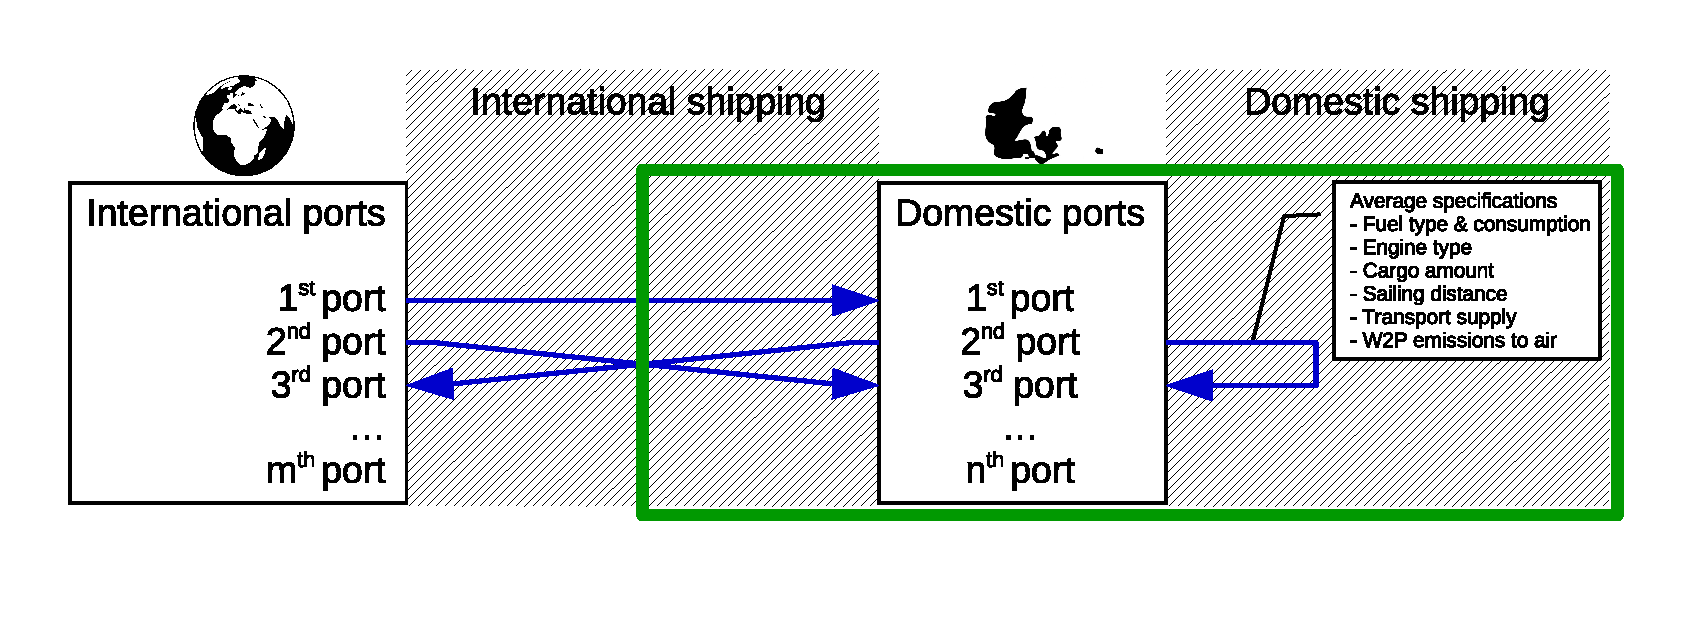
\includegraphics[width=\textwidth]{figures/model_boundary_paper.eps}
    \caption{Model boundary: The model considers the specifications inside the green box. Figure taken from \cite{Thesis2018}}
    \label{fig:model_boundary}
\end{figure}

\subsection{Model Structure}
\label{subsec:Structure}
While the core components of the model are the equations describing the objective equation and constraints of the optimisation, the pre-processing of the input data and the post-processing of the output data also constitute an important part of the modelling framework. \autoref{fig:model_boxflow} illustrates the model flow, with the white boxes representing data instances and the blue arrows representing processes. These scripts are written in Python with the pre-processing using the data package \textit{pandas}, the optimisation utilising the optimisation package \textit{pyomo} and the output processing also going to pandas \textit{mathplotlib} in order to illustrate the results as a series of plots. All scripts and raw and processed data including documentation, are available on GitHub \cite{GitHub2018}, where further development of the model takes place. To allow for barrier-free reproducibility of the presented results, the entire deployed software is open-source, while the versions of data and code deployed in this research are available at \cite{Zenodo2018}. Both are published under the GNU general public license version 3.

\begin{figure}[tbh]
    \centering
    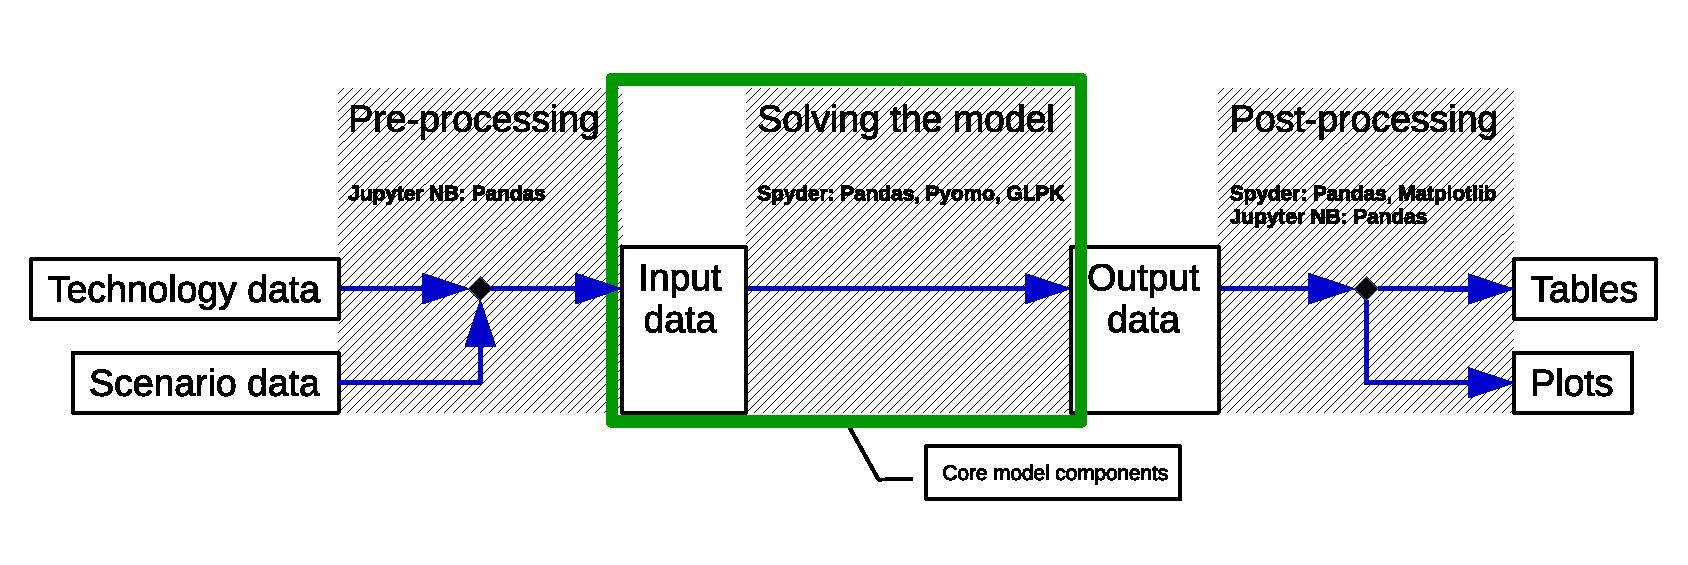
\includegraphics[width=\textwidth]{figures/model_boxflow_paper.eps}
    \caption{Model boxflow: The core model consists of the components inside the green box. (NB: Notebook; GLPK: GNU Linear Programming Kit)}
    \label{fig:model_boxflow}
\end{figure}

\subsection{Mathematical Formulation}
\label{subsec:Mat}
The problem is formulated in a linear, non-integer manner that aims to minimise the objective equation. Model variables in the first time step are initialised with data compiled for the current shipping fleet. For the following time steps, different constraints trigger the necessary investment decisions for new technologies and lead to the decommissioning of existing ships that are not in compliance with legal obligations or emissions targets. Since the objective is to minimise total system costs  (\autoref{eq:objective}), investments are interpreted as conflicting, yet inevitable actions made to cope with the constraints, such as lowering emissions to air (\ref{subsubsec:emconstraints}) and supplying the transport demand in each time step (\ref{subsubsec:tdemand}). All model variable domains are within non-negative real numbers, including zero $\left(R_{0}^{+}\right)$. The nomenclature of sets, variables and parameters used in the equations can be found in the nomenclature list (\ref{box:nomenclature}). Below, \autoref{subsubsec:obj} demonstrates the formulation of the objective equation. The entire mathematical formulation is described in \ref{app:equations}.

\subsubsection{Objective equation}\label{subsubsec:obj}
The objective equation (obj. eq.) minimises total system expenditures over all time steps and ship types (aggregated by main engine and fuel). It comprises the sum of the costs of fuel consumption, additional infrastructure and ship's capacity for all years (35 time steps in the described application). The costs of fixed assets, that is fuel infrastructure (CI) and ships (CS), are given as annuities and account only for the annual added capacities. The value of the existing amount in the start year ($finit_{t,s}$ in $T_0$) is not included in $CI$ or $CS$.
\begin{subequations}
    \begin{align}
        min. &\sum_{\forall t \in T}\sum_{\forall s \in S}\left( CF_{t, s} + CI_{t, s} + CS_{t, s} \right)\label{eq:objective}\\
        \intertext{subject to (s.t.)}
        CF_{t, s} &\geq f_{t,s} \cdot cf_{t,s}\\
        CI_{t, s} &\geq \left( iup_{t,s} - finit_{t, s} \right) \cdot li_{s} \cdot ci_{t,s}, \forall t \in T_0\\
        CI_{t, s} &\geq iup_{t,s} \cdot li_{s} \cdot ci_{t,s}, \forall t \in T_{>0}\\
        CS_{t, s} &\geq \left( sup_{t,s} - finit_{t, s} \right) \cdot ls_{s} \cdot cs_{t,s}, \forall t \in T_0\\
        CS_{t, s} &\geq sup_{t,s} \cdot ls_{s} \cdot cs_{t,s}, \forall t \in T_{>0}
    \end{align}
\end{subequations}

\glsdisablehyper
\glsaddall
\begin{table*}[h]
\begin{mdframed}
\footnotesize{
\begin{multicols}{2}
\printglossary[style=tree,type=obj]
\end{multicols}
}
\end{mdframed}
\label{box:nomenclature_obj}
\end{table*}



\subsection{Data}
\label{subsec:Dat}
The main input data for the model consists of type of fuel and of ship specifications for the initial set of the start year, as well as future options for ship technology combinations. For the fuel data, the unique identifier is fuel type, and for the ship data it is ship type. Different ship types can use the same fuel but different engine types, like internal combustion (IC), fuel cell (FC) or electric motor (EM).

\subsubsection{Fuel data}
The fuel parameters (\autoref{tab:fuel_data}) include CO$_2$ and CH$_4$ emissions factors from well-to-tank (w2t), sulphur content and the cost parameters. Costs are specified for fuel and infrastructure, as well as respective lifetimes. For fuels that are currently applied on a large scale, such as heavy fuel oil (HFO), marine diesel oil (MDO) and bio-diesel oil (BDO),  bunker index prices are used. It is assumed that these include all cost components from well to tank, including fixed costs for a sufficient supply infrastructure. Thus, in these cases the infrastructure and fuel costs are not further specified. In contrast, new fuel technology costs are divided into fixed and variable components, since sufficient supply infrastructure has not been installed as yet. If fuel upgrading is required, it is assumed that will be be done at berth to avoid additional grid investments. In the case of Denmark, the gas grid could handle any conceivable amount of natural gas and transport of upgraded biogas. Liquefied biogas (LBG) is considered a potential future carbon-based electrofuel produced from CO$_2$ and water using electricity as the primary energy source.


\subsubsection{Ship and technology data}
Ship-type input parameters (\autoref{tab:ship_data}) include emissions factors, compliance with sulphur and NO$_x$ regulations, lifetime, options for refit, costs, transport supply and application options regarding range. The amounts of fuels used today are also provided in the tables since these are applied as the starting point in the modelling, while future amounts are determined endogenously by the model.

The emissions factors for CO$_2$ and CH$_4$ only include the tank-to-propeller emissions, since the upstream emissions are already covered by the fuel parameters. Regarding sulphur and NO$_x$ compliance, Tier rating defines whether a ship is compliant with IMO NO$_x$ regulations and can thus be operated in a NECA. The old ships in the model do not have a sufficient TIER rating and thus either have to be scrapped or refitted when the regulation enters into force in 2021. New built ships are generally assumed to have a TIER 3 rating. Scrubber installations for sulphur are defined for each ship type.

Taking into account the bulk, container and tanker ship types that dominate the Danish cargo fleet,the average remaining lifetime for existing ships is eleven years, since the average age of the current fleet is fourteen years \cite[Tab.~2.2, p.~27]{UNCTAD2017}. Retrofitting an old ship to comply with new regulation may be an option to reduce costs. Currently a typical refit to comply with sulphur regulations invloves installing a scrubber for ships with internal combustion engines running on HFO. It should be noted that this results in a reduction of specific transport per fuel due to efficiency losses caused by the scrubber. Ships with internal combustion engines using HFO can also be refitted for the use of BDO, which is relatively straightforward and thus does not imply much cost. These kinds of refit do not extend the lifetime of the ship or technology, but just provide a different functionality.

Regarding the range options, only fully electric ships are restricted to radius of 500 nautical miles, equivalent to 926 km (derived from \cite{Stensvold2018a}); all others have an unlimited range.


\subsubsection{Emission budget}
\label{subsec:em_budget}
The remaining emissions budget of CO$_2$e for the temporal scope of the model is a decisive constraint in the calculation. Since there are no agreed or standardised ways of attributing GHG emissions from international shipping to countries, we have devised a method for distributing global shipping emissions and the respective remaining carbon budget to countries \ref{subsec:Scope}). By applying a global emissions budget estimate by the IPCC \cite[Tab.~SPM.3, RCP2.6]{IPCC2013} we derive the shipping budget from its annual estimated global share of GHG emissions \citet{Olmer2017}.

A comparison of global maritime CO$_2$e emissions in 2012 with Danish emissions in 2016 and its application to the global maritime budget produces a the GHG budget for Denmark (\autoref{tab:dk_em_budget}). The absolute level of Danish cargo shipping emissions of 1.2 Mt CO$_2$e in 2016 is derived from the fuel-specific emissions operation factors, multiplied by total fuel consumed in that year. The relation of global maritime emissions in 2012 to Denmarks emissions in 2016 indicates a rather over-estimated Danish budget, since global transport demand was increasing in that period \cite[Tab.~3,~p.~5]{UNCTAD2017}. Keeping the resulting emissions level constant would deplete the budgets within the next fifteen years and would allow fewer GHG emissions compared to a linear decrease from today until 2050.
\begin{table}[htb]
    \centering
    \begin{tabular}{llrr}
        \toprule
         & Unit & CO$_2$ emissions & References \\
         \midrule
         Global budget & $\left[Mt\right]$ & 510000 & \cite{IPCC2013} \\
         Global maritime budget share & $\left[\%\right]$ & 3 & \cite{Olmer2017} \\
         Global maritime budget & $\left[MT\right]$ & 15300 &\\[1.5ex]
         Global maritime emissions in 2012 & $\left[Mt\right]$ & 961 & \cite{Smith2014} \\
         Danish maritime emissions in 2016 & $\left[Mt\right]$ & 1.2 & \cite{Kristensen2012,Eurostat2018,Wisdom2017} \\
         Danish maritime emission share & $\left[\%\right]$ & 0.125 &\\[1.5ex]
         Danish budget & $\left[Mt\right]$ & \textbf{19.12} & \\
         \bottomrule
    \end{tabular}
    \caption{Derivation of CO$_2$e emission budget from global to Danish level.}
    \label{tab:dk_em_budget}
\end{table}


\subsection{Scenarios}
\label{subsec:Sce}
In general, all scenarios except the business-as-usual (BAU) and IMO scenarios are modifications of the reference scenario's input parameters. See \ref{app:tables} or \cite{Thesis2018} for more details about the assumptions made for each of these scenarios. The reference scenario and its modifications all comply with the restrictions on the carbon budget. In the variations, one or a cluster of parameters are changed in a ceteris paribus manner and by the same percentage. If appropriate, changing rates are clustered due to the coupling effects. For example, electrofuel cost parameters all change in the same way in the respective variation scenarios, as they all depend primarily on electricity. In Addition, the transport demand variation (TDV) scenario illustrates the possible effects of a transport demand decreasing by 30\% by 2050, otherwise it is kept constant.

\subsubsection{Scenario data}
How the cost and other parameters develope is decisive for the model results. To make the assumptions behind this transparent, the variations are expressed as percentage change rates from 2016 to 2050 (\autoref{tab:ref_rates}). Derived from that number, equal annual changing rates are applied. \autoref{tab:ref_rates} shows the parameter changes and thus the future development of the reference scenario.

Other decisive parameters are bio-fuel availability and transport demand. Bio-fuel availability increases from 0 \% in 2016 to 40 \% in 2050 in relation to total fuel consumption in 2016 \cite{DEA2016}. The transport demand stays constant based on \cite[p.~18]{ITF2018} and \cite[p.~19]{Rex2017}.


\subsubsection{Scenario overview}
\autoref{tab:scn_overview} provides an overview of the fourteen scenario variations and the respective modified parameters. The extent to which the respective scenario parameters are modified is given alongside the results in \autoref{sec:Results}.

\begin{table}[thb]
    \centering
    \resizebox{\textwidth}{!}{%
    \begin{tabular}{lll}
        \toprule
        Scenario & Description & Modified \\
        & & parameters \\
        \midrule
        REF     & Reference scenario, based on literature & - \\
        REF(mp) & Reference scenario  + methane leakage phaseout & em \\
        BAU     & Business as usual & eb, et \\
        IMO     & International Maritime Organization & eb, et\\
        TDV     & Transport demand variation & tdtotal \\
        BATW    & Cost variation of battery and wind & cf, ci, cs \\
        BDO     & Cost variation of bio-diesel oil & cf \\
        CH3OH   & Cost variation of methanol & cf, ci, cs\\
        H2      & Cost variation of hydrogen & cf, ci, cs \\
        LBG     & Cost variation of liquefied bio-methane & cf, ci, cs \\
        LBG(mp) & Cost variation of liquefied bio-methane + methane leakage phaseout & cf, ci, cs, em \\
        LNG     & Cost variation of natural gas & cf, ci, cs \\
        LNG(mp) & Cost variation of natural gas + methane leakage phaseout & cf, ci, cs, em \\
        NH3     & Cost variation of ammonia & cf, ci, cs \\
        \bottomrule
    \end{tabular}}
    \caption[Scenario overview]{Scenario overview with description and modified parameters. For additional information about scenarios see \cite{Thesis2018}. (cf: fuel costs; ci: infrastructure costs; cs: ship costs; eb: emission budget; em: CH$_4$ emissions; et: emission target; tdtotal: total transport demand)}
    \label{tab:scn_overview}
\end{table}

\section{Results and Discussion}
\label{sec:Results}
In the business-as-usual scenario (BAU) no GHG regime is in place. Although SO$_X$- and NO$_X$-restrictions are applied, no major change in fuel usage can be detected. \autoref{fig:BAU} displays fuel consumption and cumulative CO$_2$e emissions under BAU. It shows that scrubbers, not fuel switching, are the most cost-efficient solution if no GHG restrictions are implemented. Applying the IMO goal to halve climate emissions from shipping by 2050 does not lead to significant changes except for a minor switch to BDO instead of HFO (\autoref{fig:IMO}). By comparison, the climate emissions budget restriction in the reference scenario  results in a significant fuel switch, with hydrogen in fuel cells and BDO with scrubber in internal combustion engines mainly being chosen (\autoref{fig:REF}). The comparison shows that, without any kind of restriction on climate emissions, total cumulative emissions are twice as high and the IMO's plans do not have a significant impact. 

\begin{figure}
    \centering
    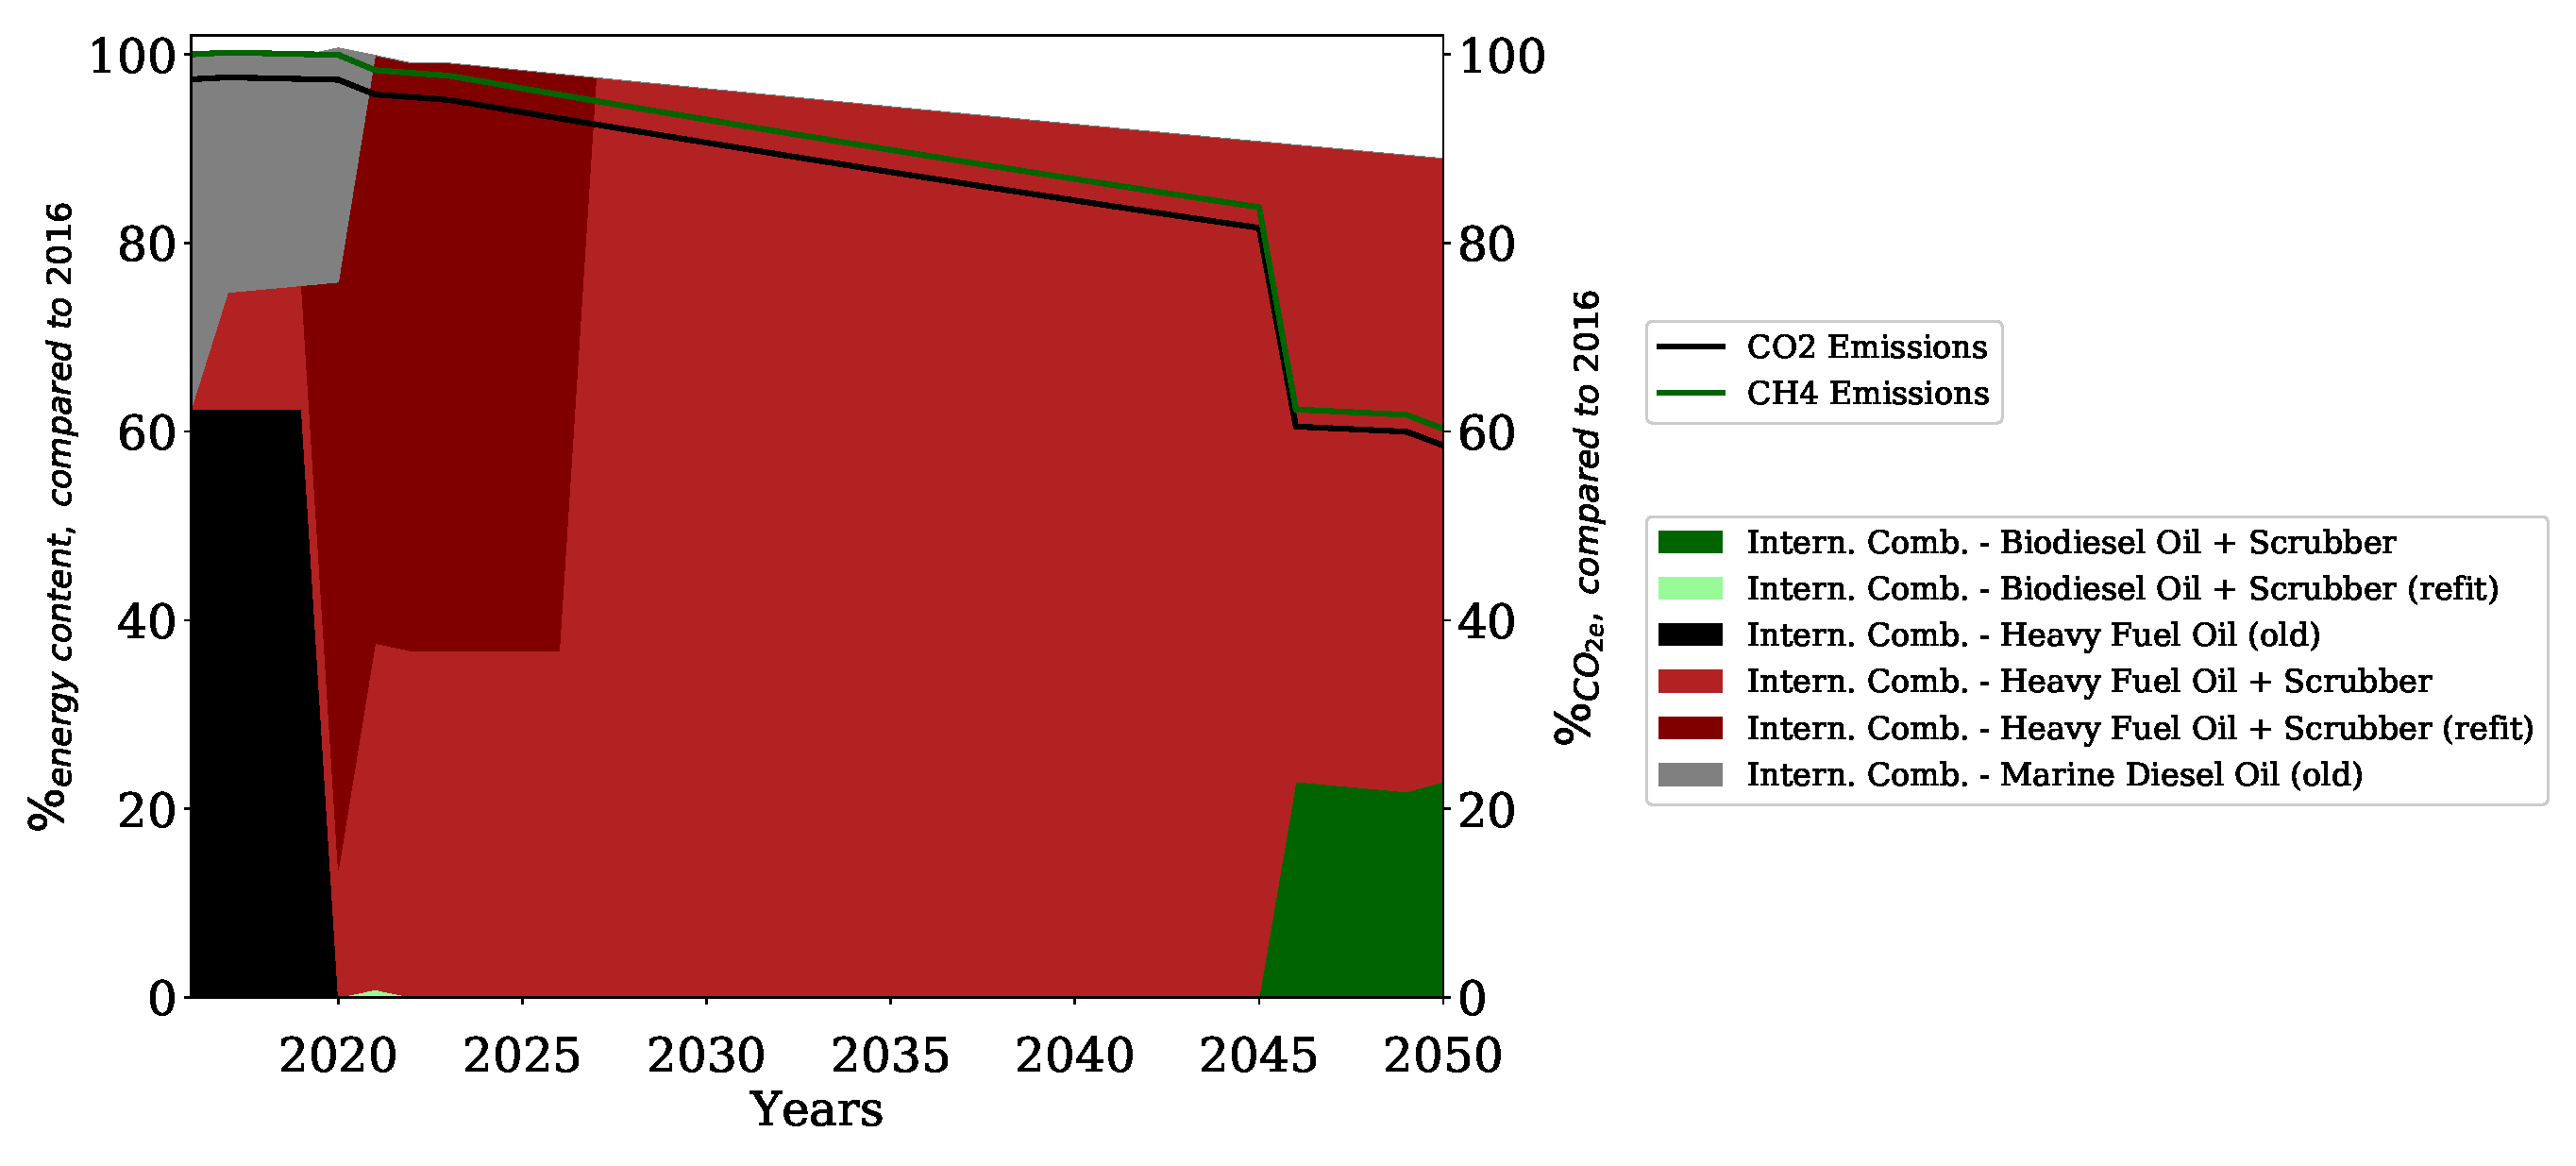
\includegraphics[width=\textwidth]{figures/IMO_fuels_emissions.eps}
    \caption{Fuel consumption (y-axis left) and cumulative emissions (y-axis right) in the IMO scenario, applying the climate emission target of the International Maritime Organisation for 2050.}
    \label{fig:IMO}
\end{figure}

\begin{figure}
    \centering
    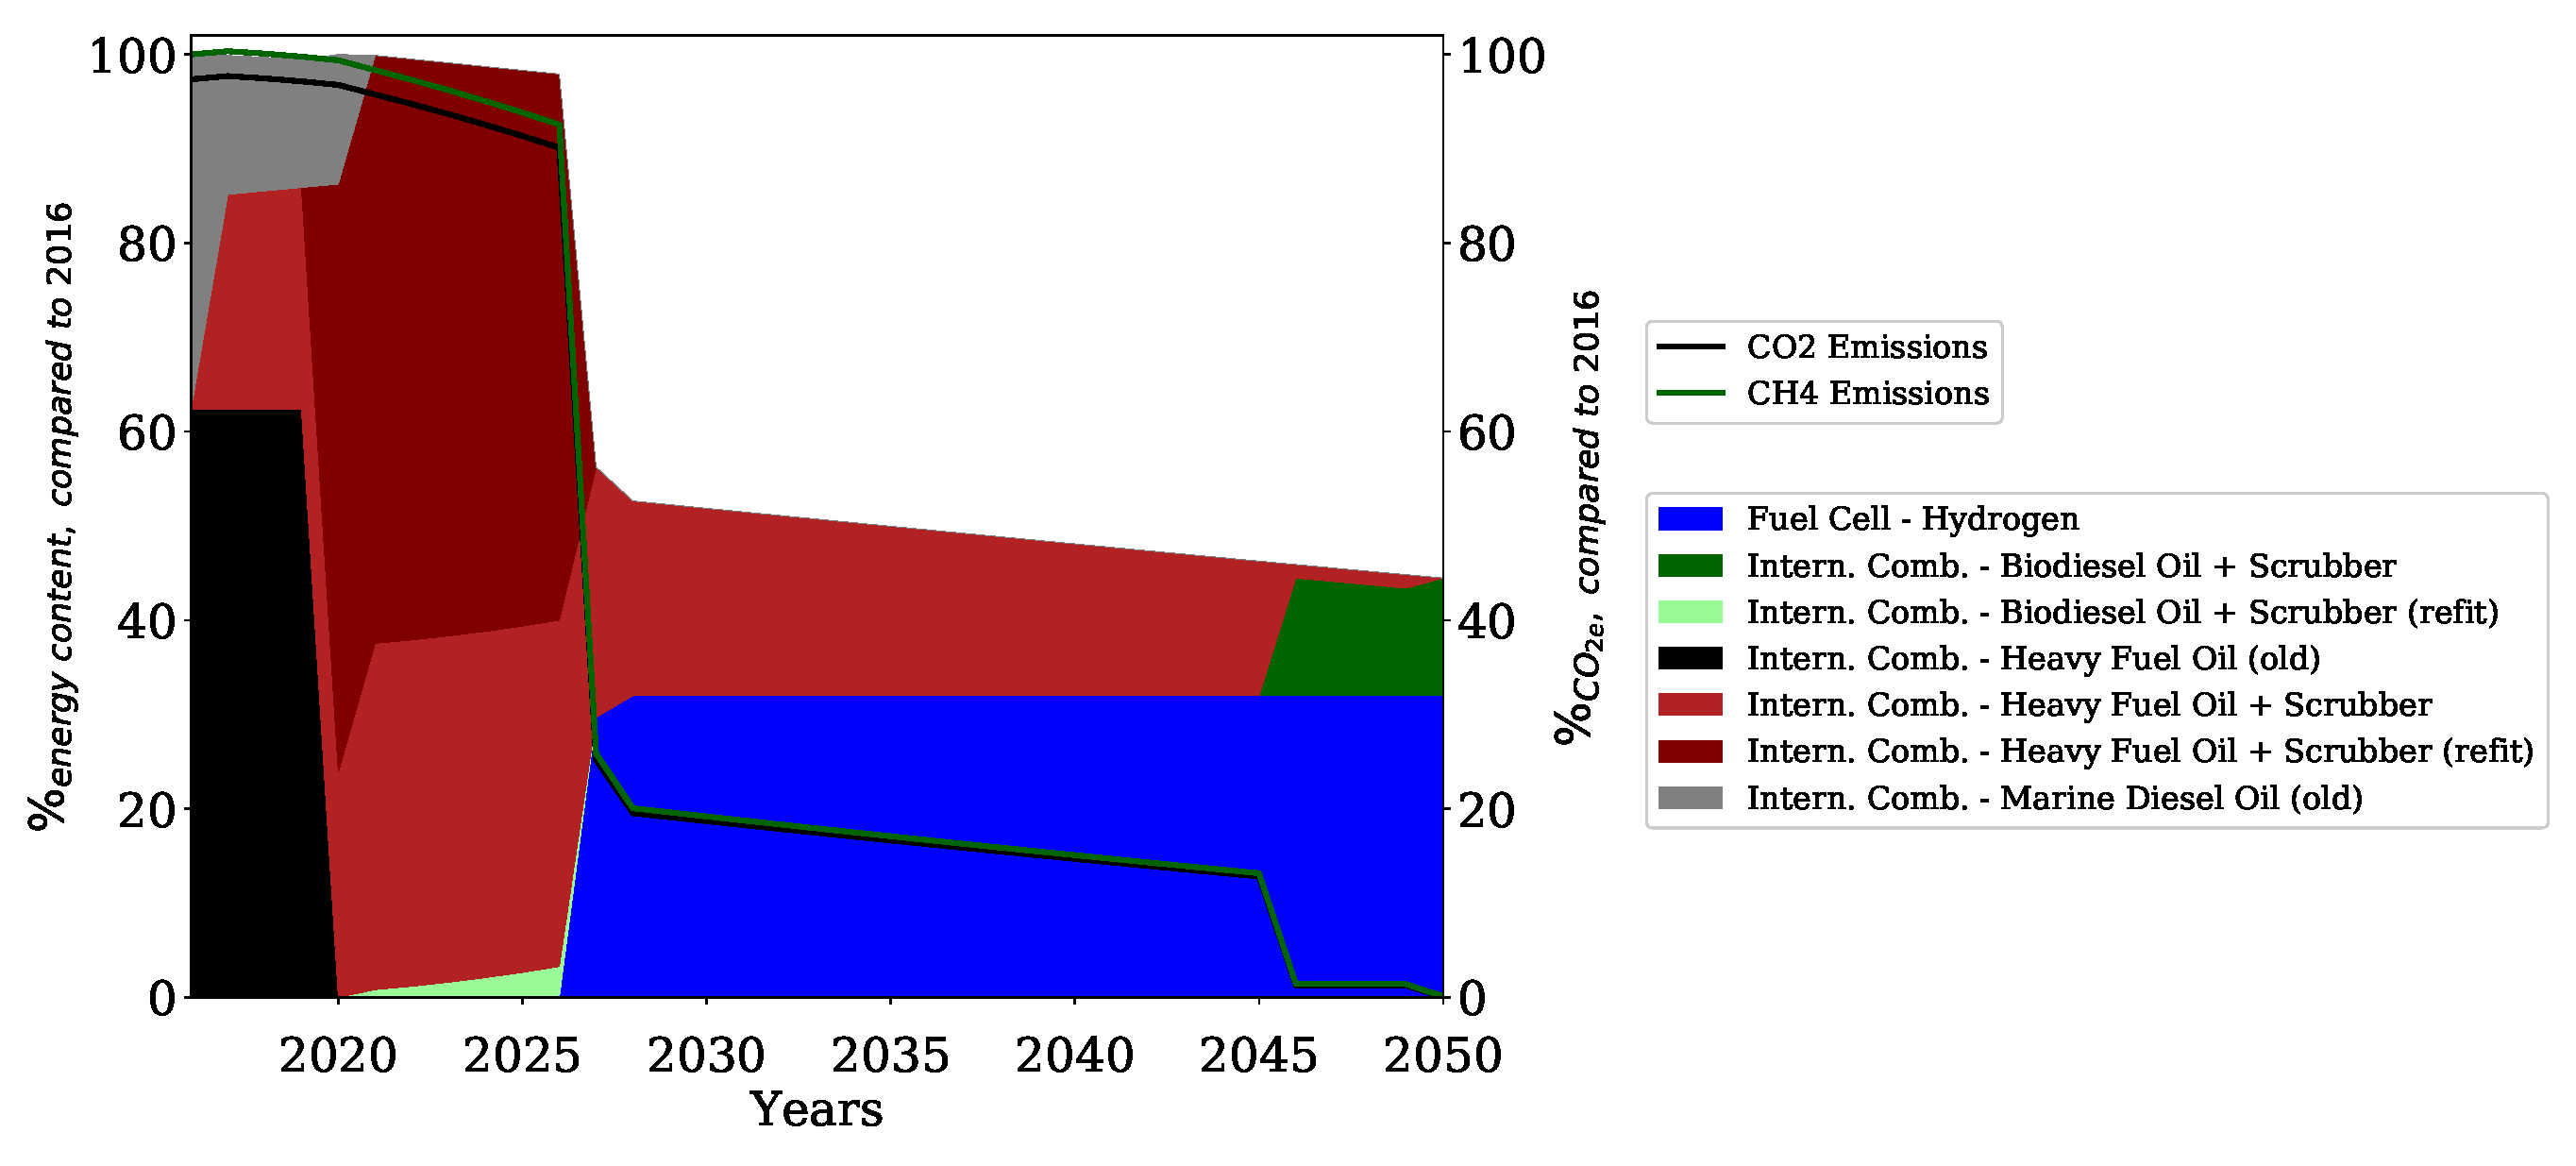
\includegraphics[width=\textwidth]{figures/RS_fuels_emissions.eps}
    \caption{Fuel consumption (y-axis left) and cumulative emissions (y-axis right) in the reference scenario with a limited carbon budget.}
    \label{fig:REF}
\end{figure}

Due to the high level of uncertainty of cost developments for the infrastructure, fuel and propulsion technology of different marine fuel options, we apply a wide range of cost variations to test for their effects on fuel composition. The results are summarised in \autoref{fig:costVariation}. Depending on the cost rate change of a specific fuel technology (x-axis), while all other parameters are kept constant, the share of total fuel consumption from 2016-2050 (y-axis) changes significantly. The black dashed line at a cost rate change of zero represents the reference scenario. Already at a -10\% change in cost rate (including fuel, ship and infrastructure costs), methanol and ammonia respectively gain relevance, reaching a dominant role at a -20\% cost change rate. Thus, if the costs of either methanol or ammonia drop by -20\%, these would take over the role of hydrogen as the main renewable fuel of the future. These scenario variations are illustrated in \autoref{fig:Ammonia} and \autoref{fig:Methanol}.

\begin{figure}
    \centering
    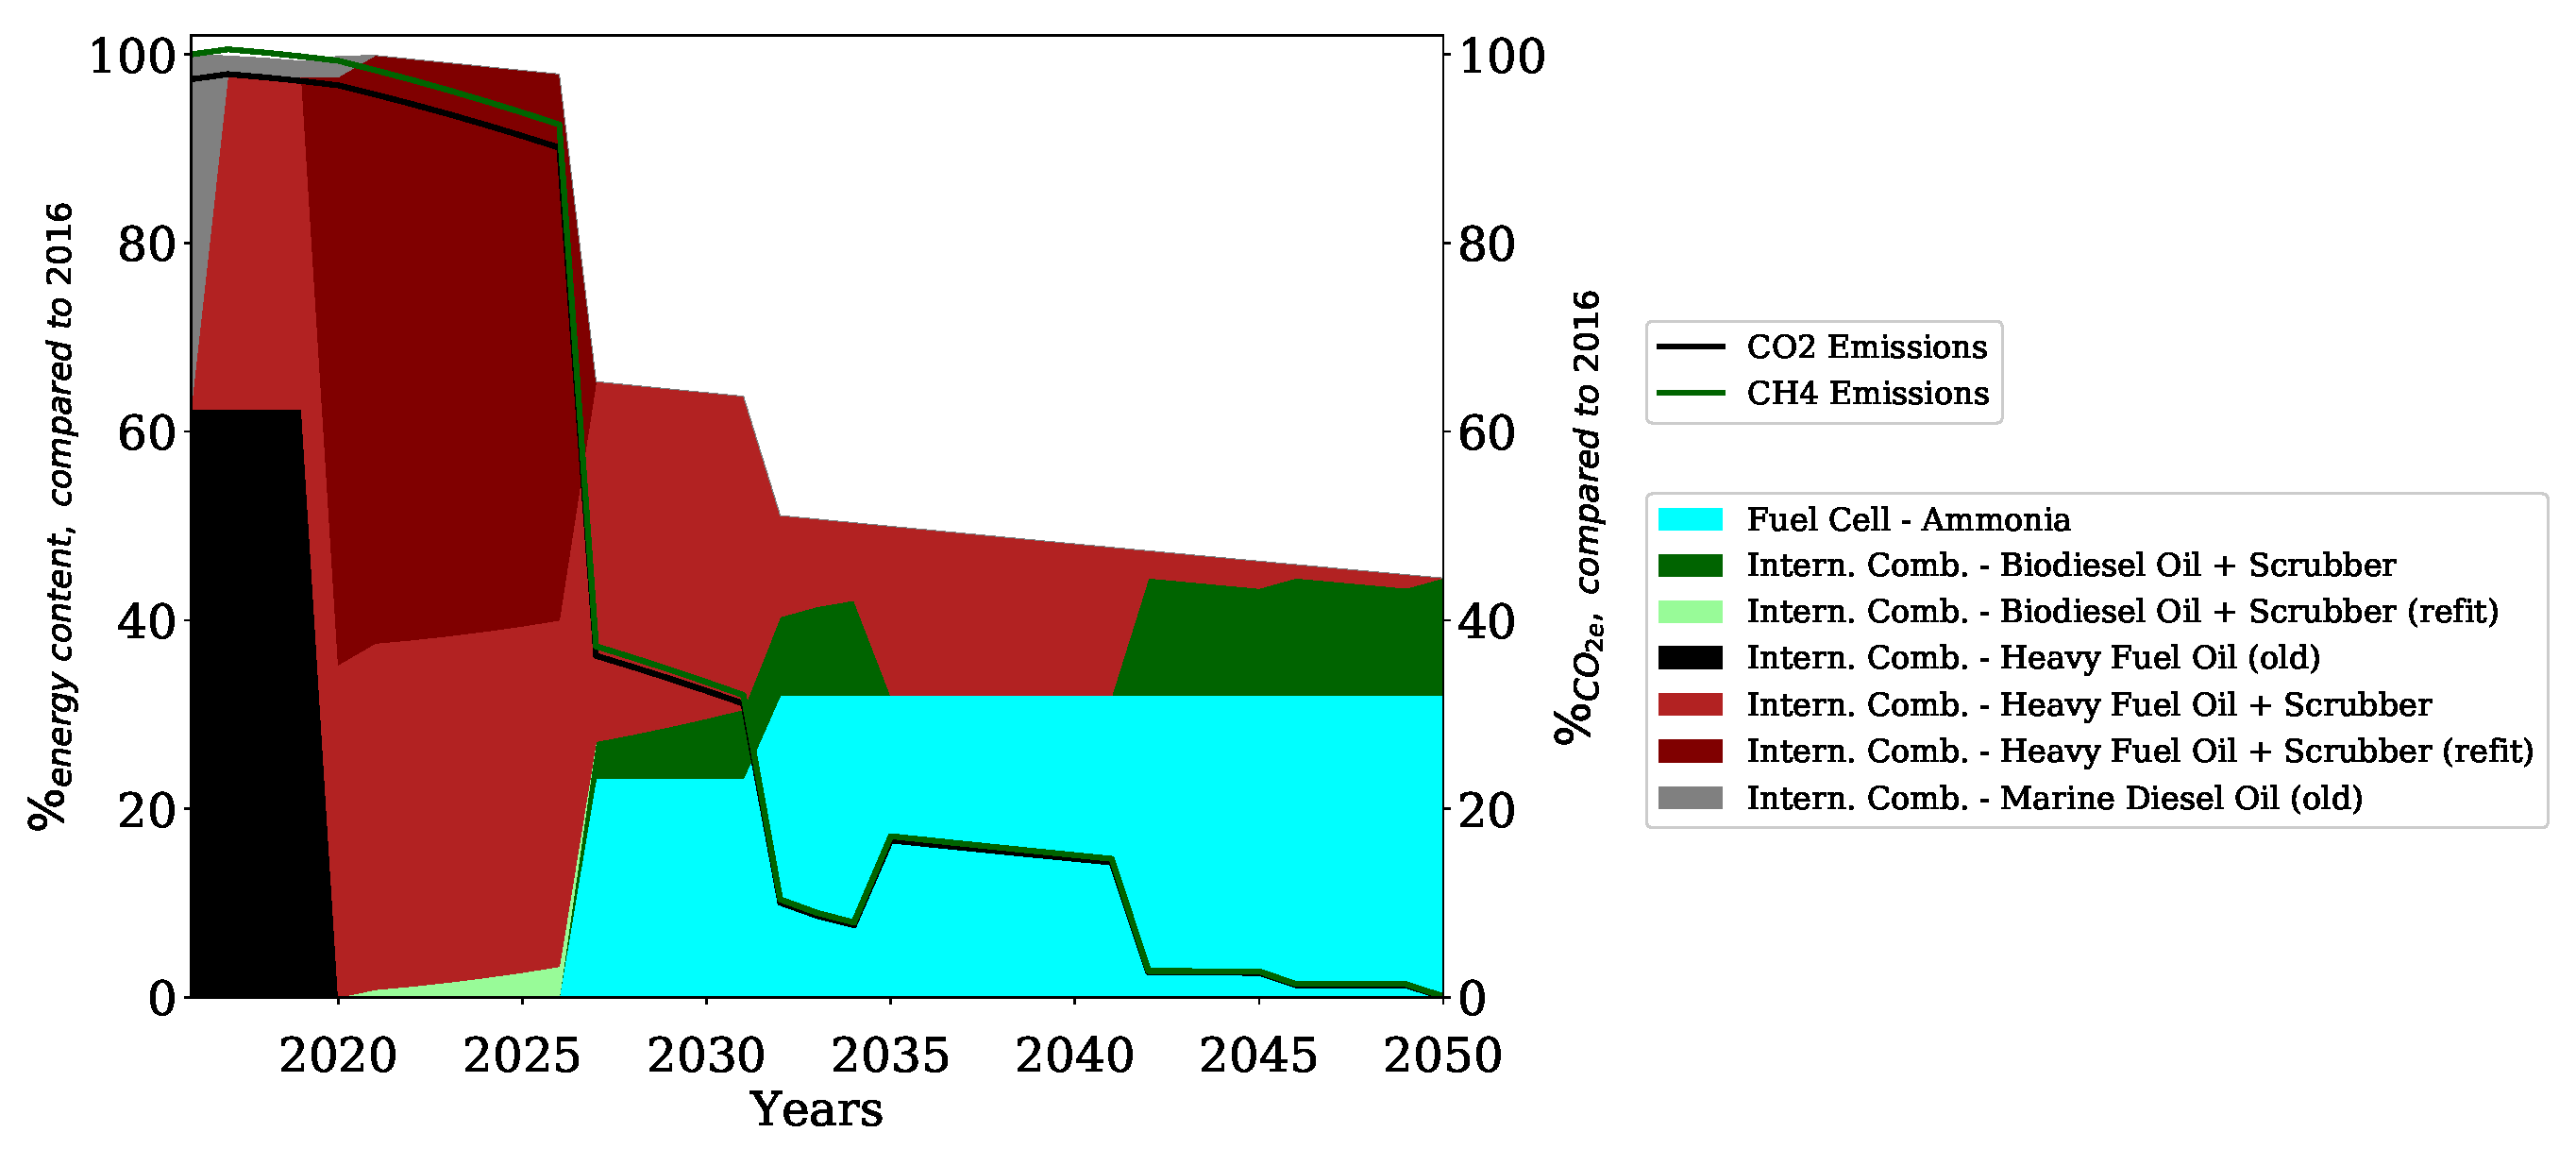
\includegraphics[width=\textwidth]{figures/NH3_fuels_emissions.eps}
    \caption{Fuel consumption (y-axis left) and cumulative emissions (y-axis right) in the ammonia scenario (NH3, r-20) with a limited carbon budget.}
    \label{fig:Ammonia}
\end{figure}

\begin{figure}
    \centering
    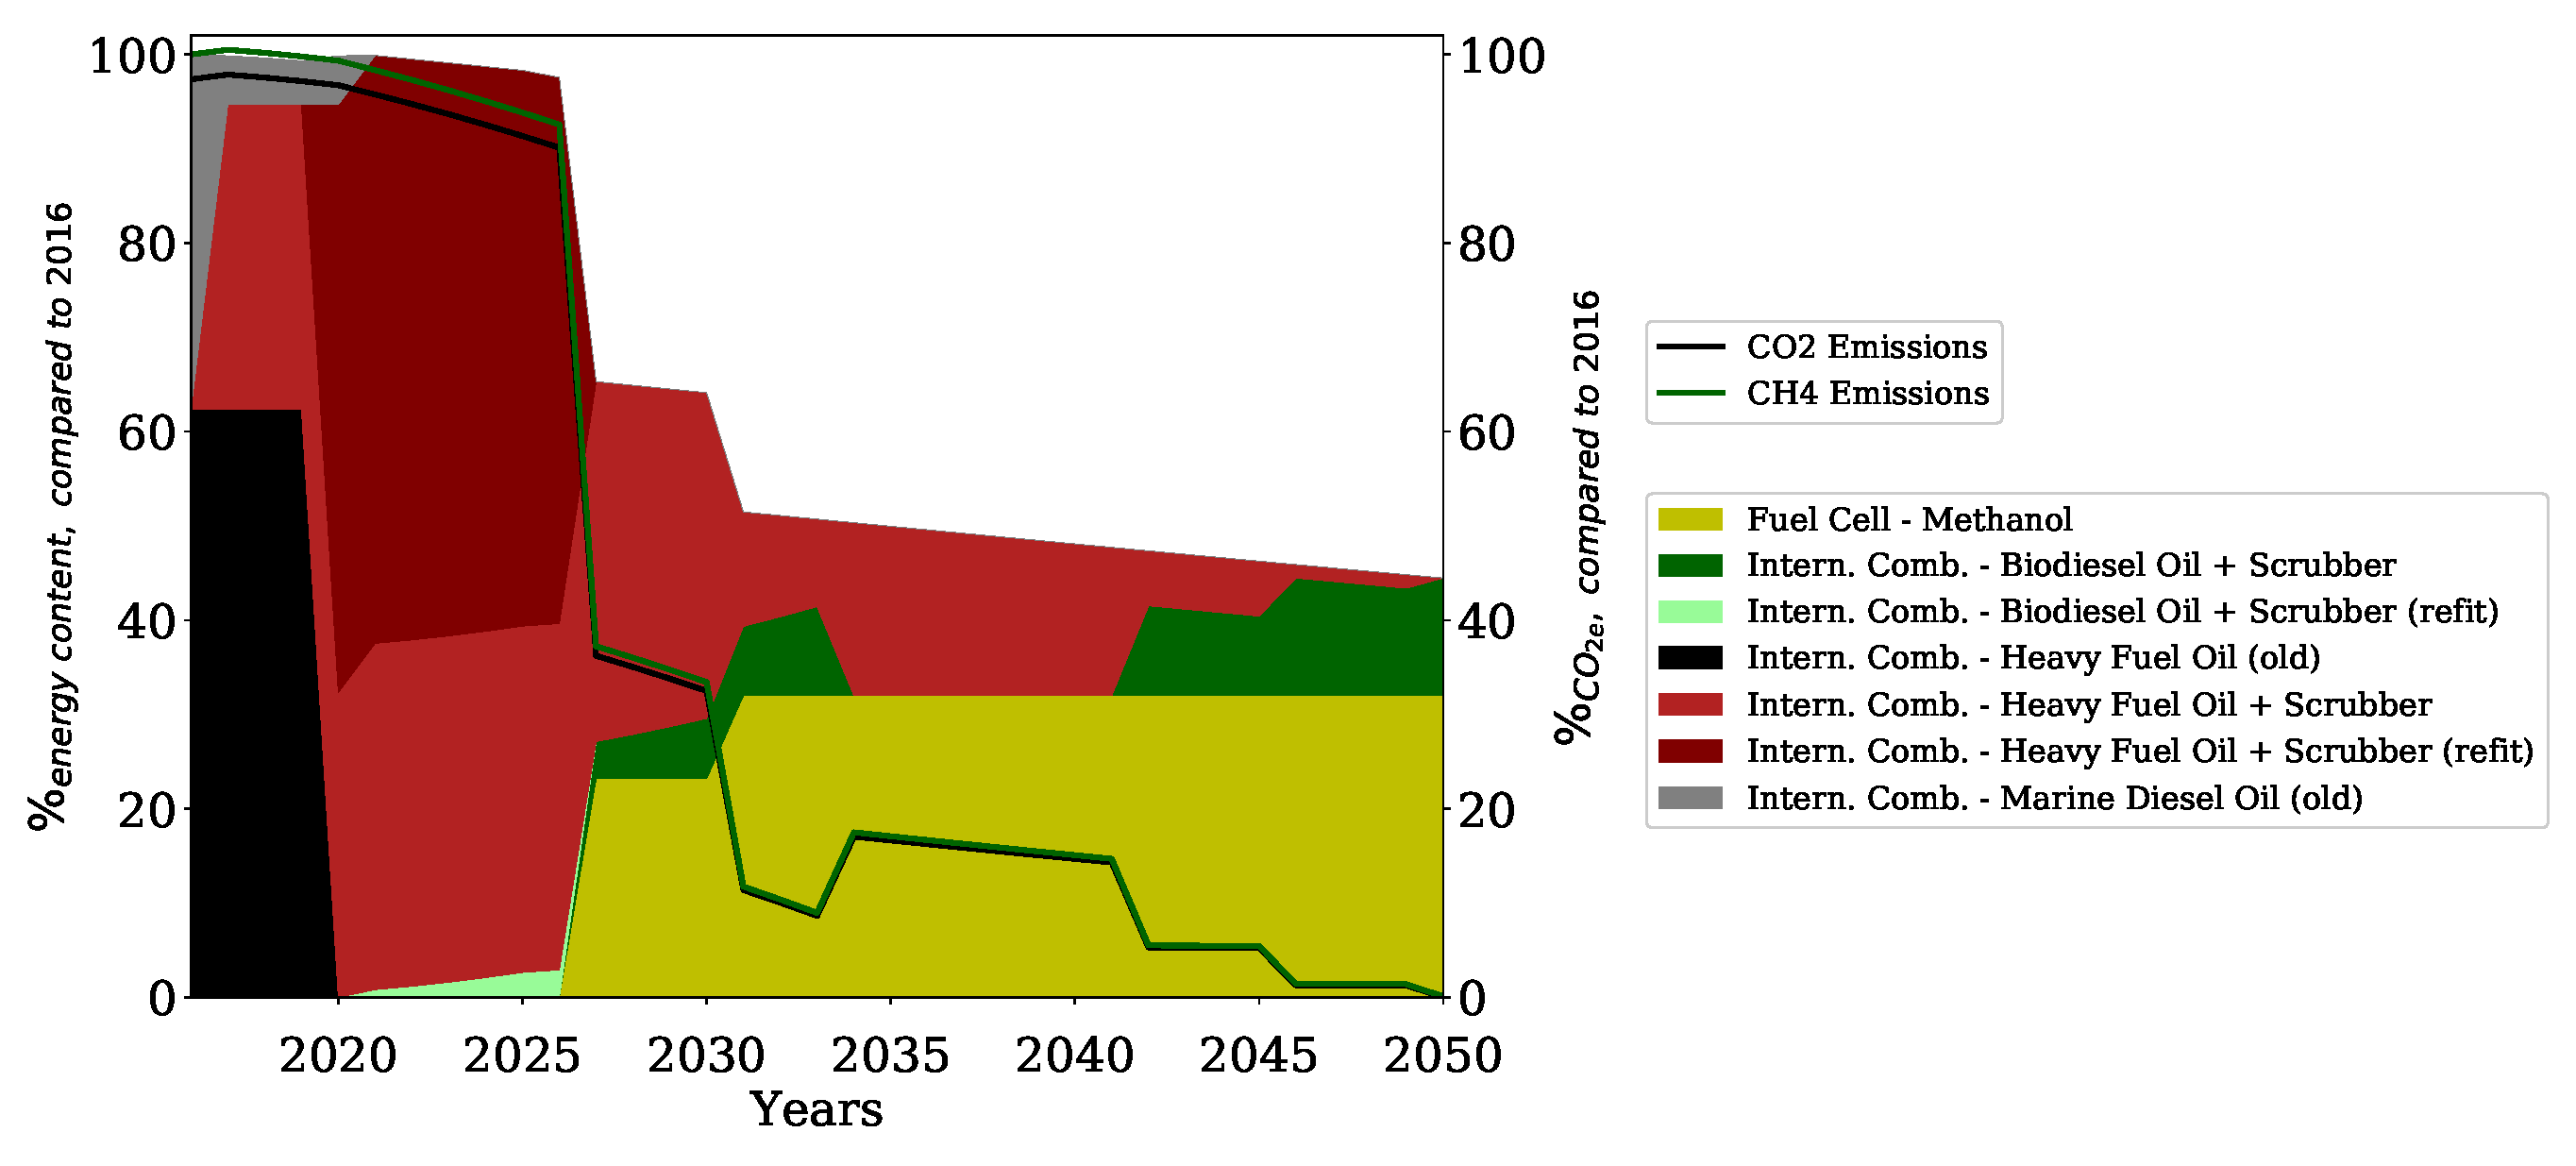
\includegraphics[width=\textwidth]{figures/CH3OH_fuels_emissions.eps}
    \caption{Fuel consumption (y-axis left) and cumulative emissions (y-axis right) in the methanol scenario (CH3OH, r-20) with a limited carbon budget.}
    \label{fig:Methanol}
\end{figure}

For LBG, how the methane leakage problem develops is of outstanding importance. Under the assumption that methane leakage can be coped with until 2050 (dashed line in (\autoref{fig:costVariation}) with a cost reduction of -40\% (\autoref{fig:LBG}), LBG is close to hydrogen, methanol and ammonia as the choice to be the dominant fuel by 2050. Conversely, not only would LNG require methane leakage to be phasd out, but a very favourable cost development would also play a major role.

Sailing cargo ships, driven by a combination of wind and electricity from batteries seem to be cost-efficient only in the case of a very strong fall in costs. However, the influence factors have more dimensions than just the pure battery and ship costs. In this model, it is assumed that one third of the propulsion of wind driven ships is still done by electricity. For long-distance cargoes, this is mainly a matter of using the engine for manoeuvring into and out of the harbour. The share of wind and potentially additional solar input can be significantly increased, thus reducing the required battery and electricity costs. Thus the conditions of our model's application are rather unfavourable for wind propulsion.

For comparison, total fuel use in all scenarios for 2016-2050 is displayed in \autoref{fig:AllFuelTotal}, as is fuel composition in the target year of 2050 in \autoref{fig:AllFuel2050}. A general increase in efficiency can be seen for all carbon budget scenarios. Due to higher operational tank-to-propeller efficiencies and thus higher Tkm/GJ fuel rates, less fuel is spent in the carbon budget scenarios. Except in the case of the transport demand scenario, all scenarios supply the same transport demand.

\noindent
\begin{minipage}[t]{0.49\textwidth}
    \centering
    \captionsetup{justification=centering}
    \captionof{figure}{Total fuel use from 2016-2050}
    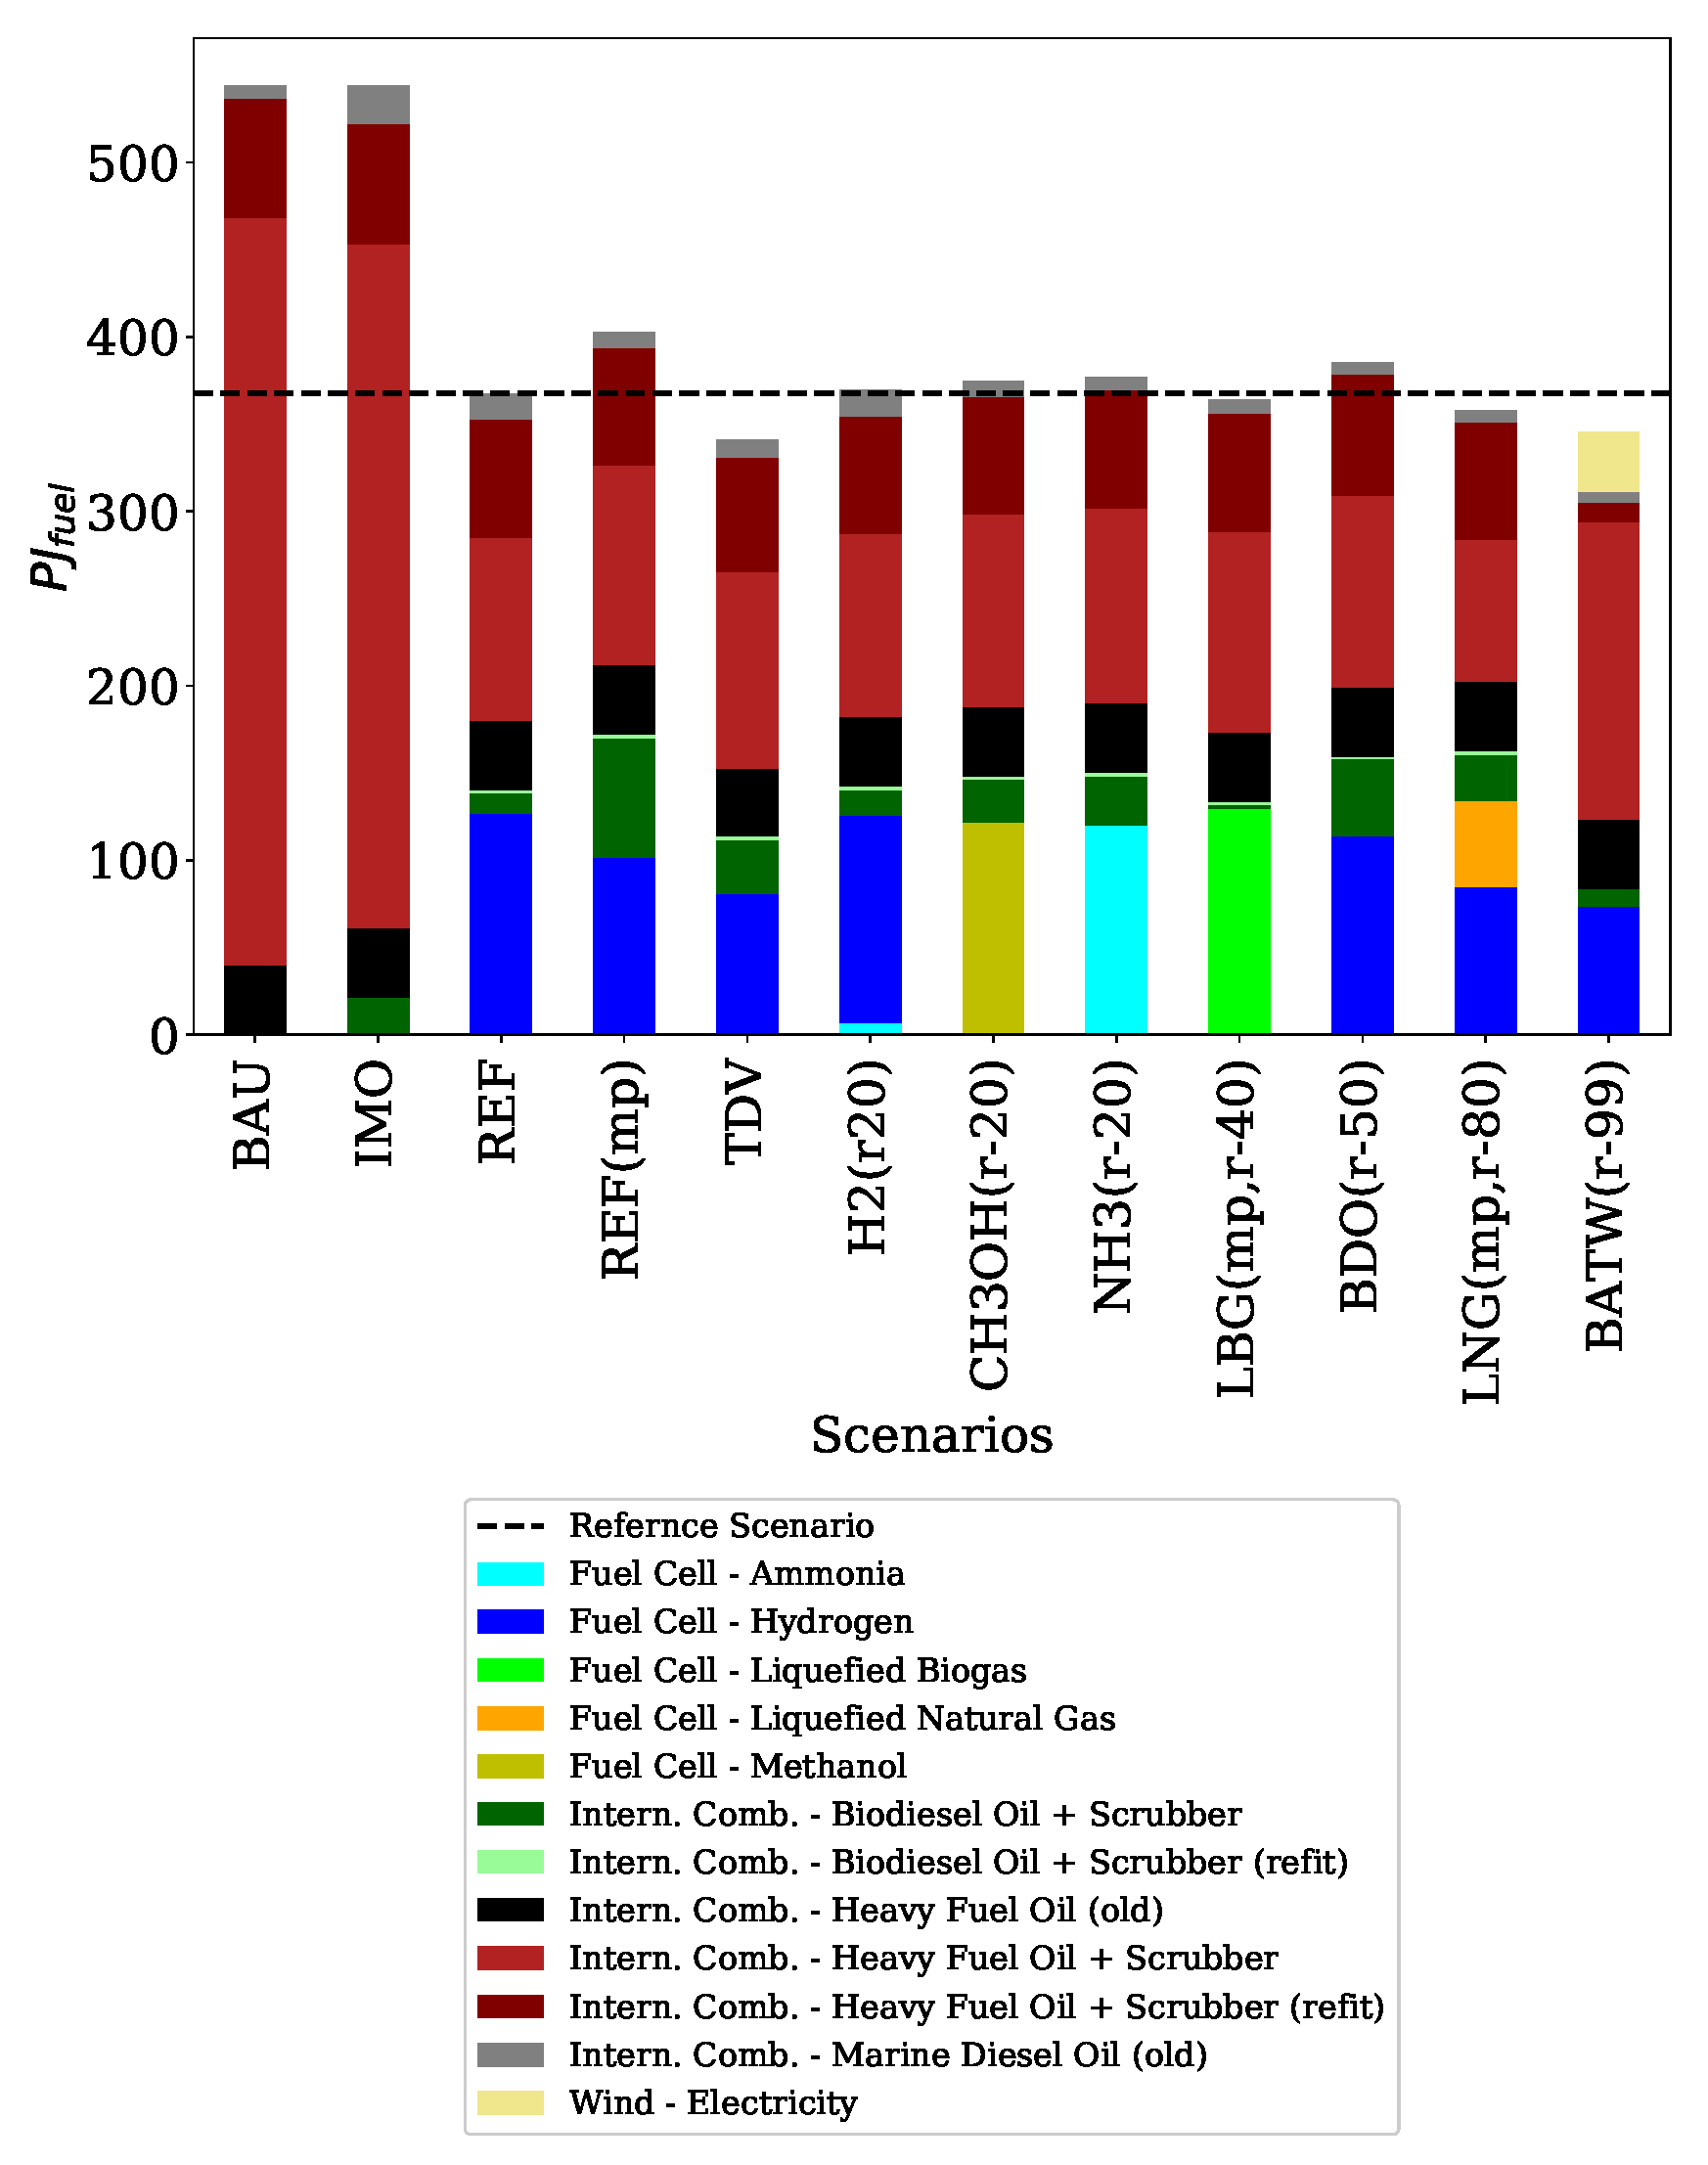
\includegraphics[width=.95\textwidth]{figures/AllFuelTotal.eps}
    \label{fig:AllFuelTotal}
\end{minipage}
\begin{minipage}[t]{0.49\textwidth}
    \centering
    \captionsetup{justification=centering}
    \captionof{figure}{Fuel composition in 2050}
    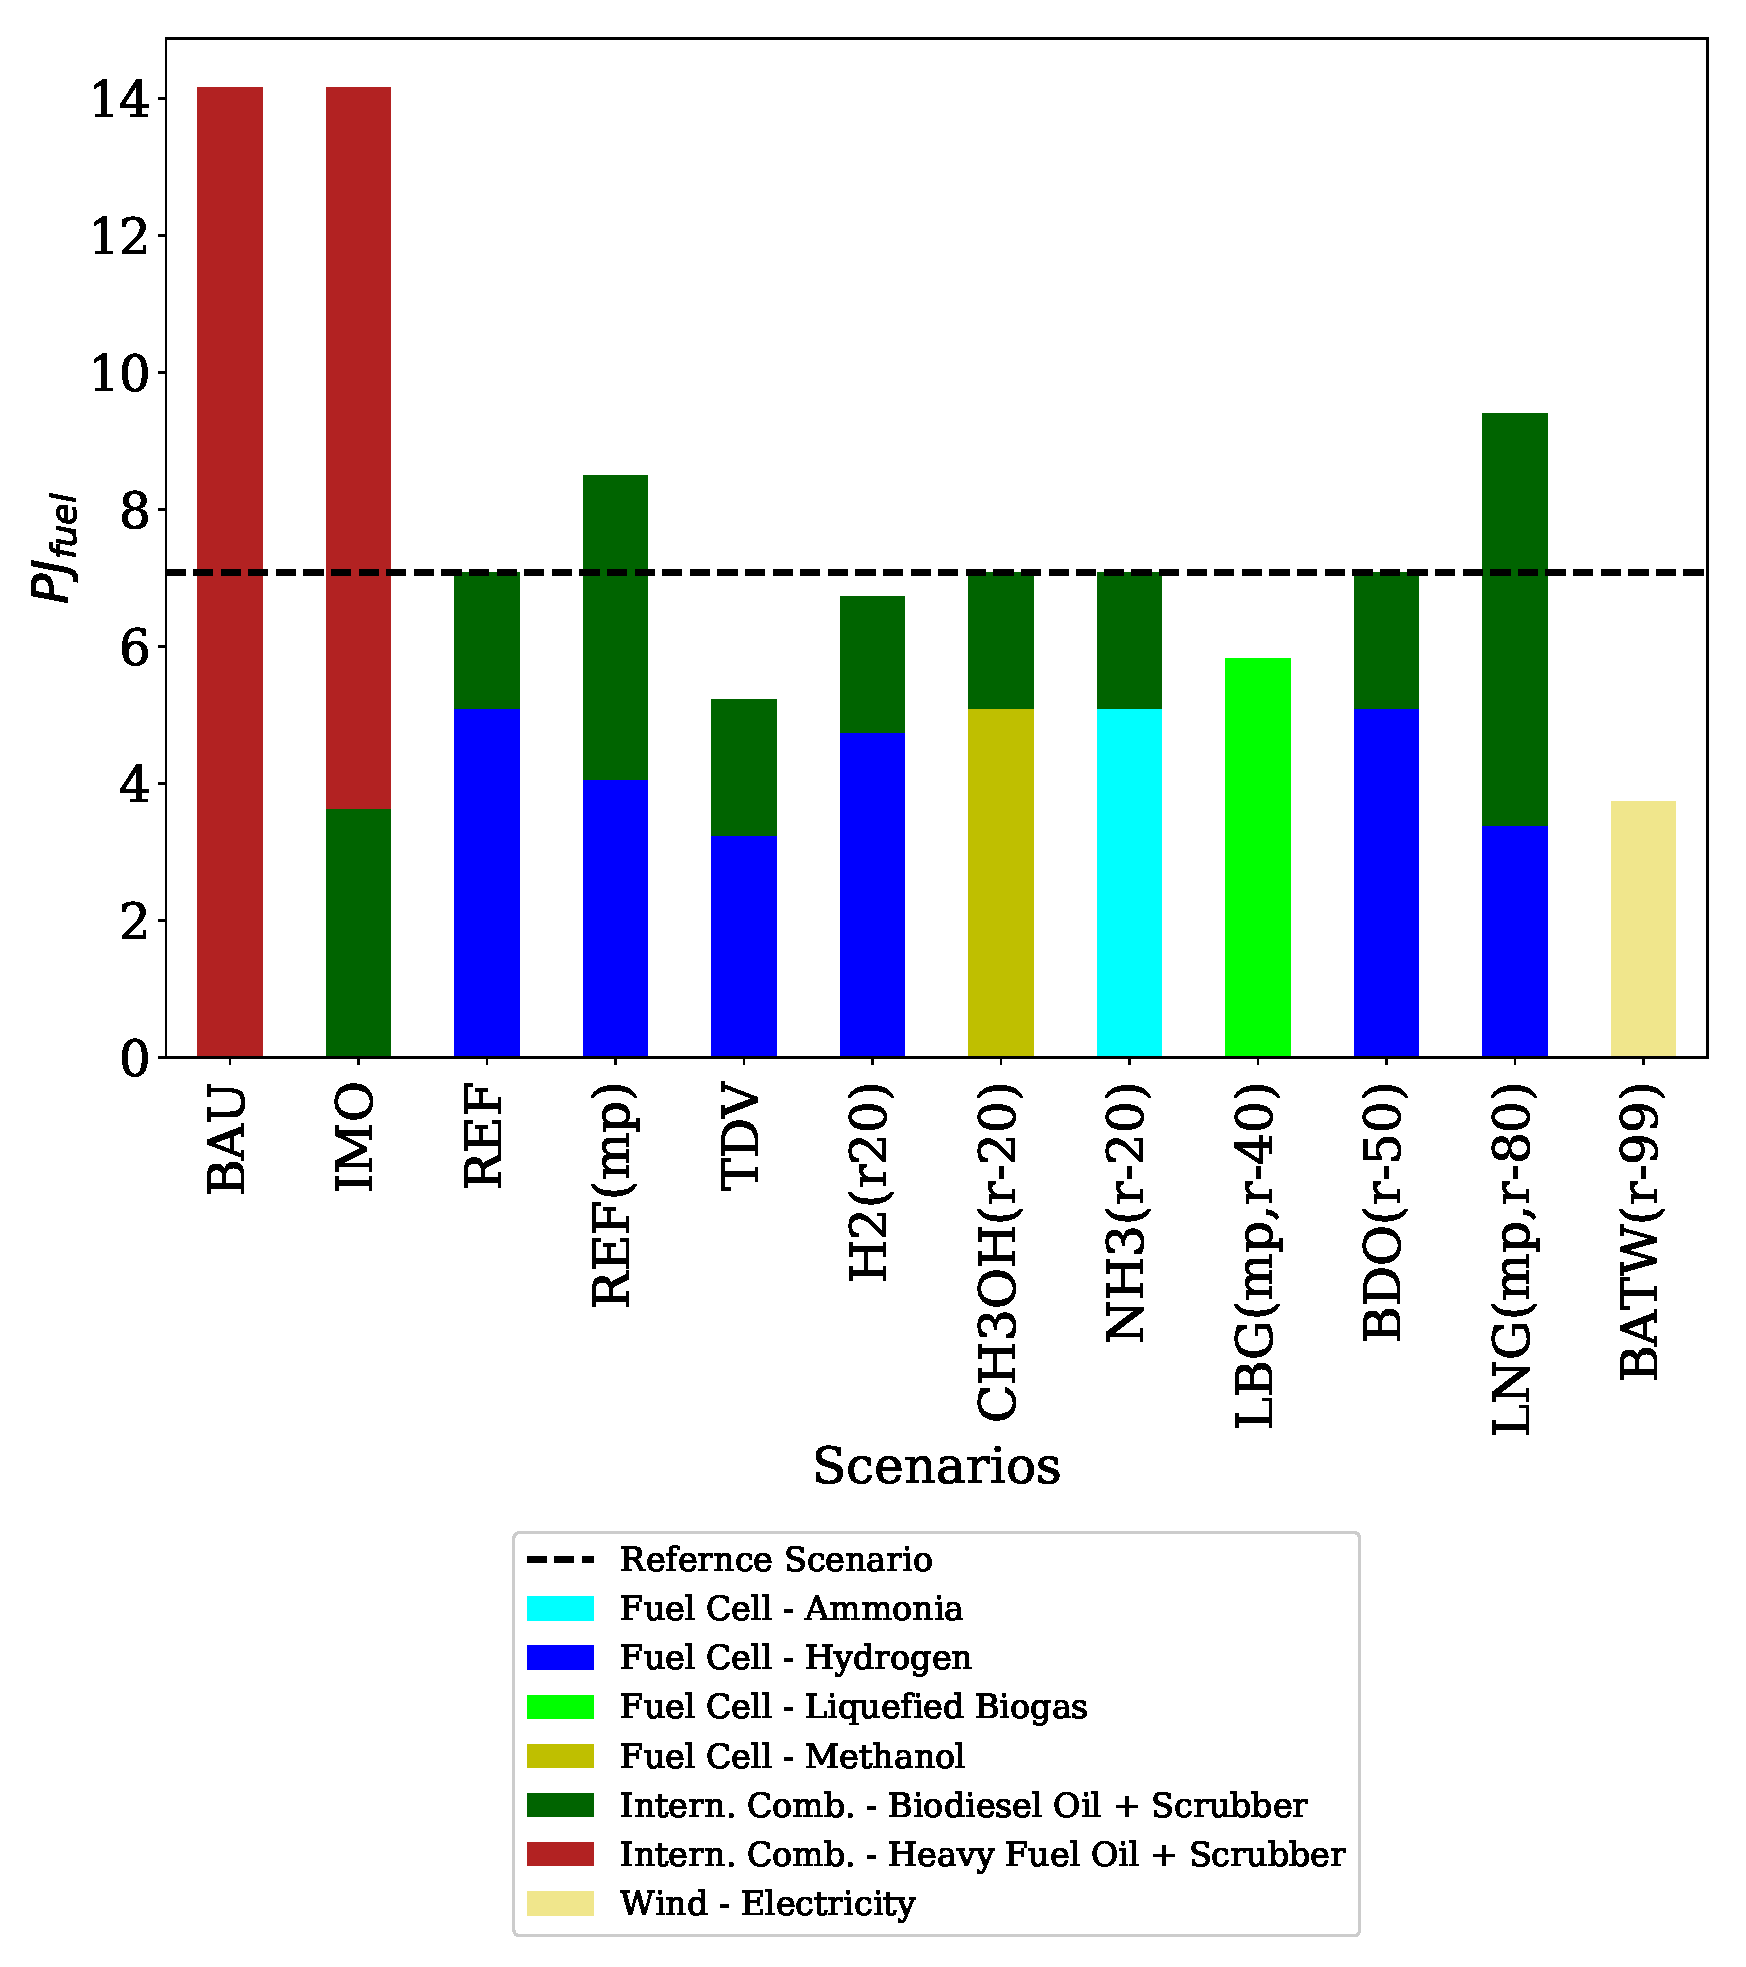
\includegraphics[width=.95\textwidth]{figures/AllFuel2050.eps}
    \label{fig:AllFuel2050}
\end{minipage}\\ %[0.75cm]

Derived from the cost differences for fuel, ship and infrastructure, a carbon price in the range of 350--450 \euro$_{2016}$/ton CO$_2$e would be required for a renewable transition to the Danish shipping sector. There are no directly comparable studies, but, to put our results in perspective, \citet[p.197]{Raucci2017} reports similar prices of around 430 \$/ton CO$_2$ for a global transition with a global shipping carbon budget twice as high as in our case. In that setting, he concludes that hydrogen requires an emissions price of 1400 \$/ton CO$_2$ to become an economic option. In contrast, a global study of country- and sector-wise CO$_2$ abatement costs \cite{OECD2016} represents the lower range: although shipping is not included, road transport is indicated at about 200 \euro/ton CO$_2$. Specific costs for climate emission-abatement costs in shipping can be expected to be higher than that, since shipping poses special challenges due to its high range requirements. More specifically regarding CO$_2$ abatement costs for shipping, \citet{DNVGL2017}, assumes costs in the range of 150--200 \euro/avoided ton CO$_2$ if using LBG, methanol based on renewables, or BDO. In reality it can be challenging for a single country to introduce a carbon price on its own, and the analysis should be scaled at an appropriate level. Thus, the numbers provide an indication of the upper boundary of a necessary worldwide carbon price.

The model code and most of the data references and pre-processing can also be applied to other countries, especially in Europe. However, since shipping is global in scope, the Danish case study already gives a good indication of the fuel shares chosen for a cost-optimal path to carbon neutrality in 2050 for worldwide shipping. Conditions for shipping are similar, as the basic parameters, namely technology, fuel and infrastructure costs are considered at world prices rather than at prices reflecting local particularities. 

Compared to other sectors, like electricity and heat, these mitigation costs per ton of CO$_2$e seem high, but several points need to be taken into account. First, our results can be interpreted as indicating the upper cost boundary: all potential technologies are considered applicable today, and developments in other sectors applying similar technology options could further decrease costs, while additional alternatives might also evolve. Second, as shown in the demand reduction scenarios, any decrease in transport demand would save costs even beyond the proportional savings. This is due not only to fuel savings (proportional) but also to avoided investments in new ships (disproportionate). A decrease in transport demand especially has an effect in the period, in which new investments in ships are required and  costs can be avoided over-proportionally. Note that the technological progression of renewable energy sources in the electricity sector has a strong influence on the costs in alternative green shipping (assuming hydrogen or ammonia). Third, although refits and hybrid solutions have not been considered to any extent in respect of the model's functionality, they could decrease costs further and ease the shift to different fuels.

Transport costs in the BAU scenario amount to roughly 3 \euro$_{2016}$/ton cargo. For climate compatible pathways they are likely to more than double. With \citet[p.~50]{UNCTAD2015} reporting average transport costs of around 5 \euro/ton and including more detail, our results seem to be acceptably precise. Further, \cite[p.~55]{UNCTAD2015} states that transport costs in developed countries are equal to 7 \% of the cargo's import value. Under the assumption of an equal share in the BAU scenario, cargo import values for climate compatible pathways would increase by 6 -- 8 \%.
Thus, costs could fall lower during the transition, but the question is also whether mitigation costs need to be taken into account. Co-benefits like reduced air pollution were not quantified on a monetary basis in the model and were thus not part of the optimisation. However, these could have essential health benefits, maybe even achieving mitigation gains instead of mitigation costs.

The necessary transition will not happen under current market conditions. Regulation is required urgently to bring shipping on to the pathway to carbon neutrality in 2050, in line with the Paris Agreement. A carbon budget for shipping worldwide, broken down by countries, is a viable option to consider. In addition, more research into alternative fuels and technologies, as well as solving crucial questions regarding issues in respect of security, infrastructure and methane leakage, will be important contributions to implementing the transition to climate-neutral shipping by 2050. 


\section{Conclusion}
\label{sec:Conclusion}
The achievement of CO$_2$e-neutrality in the shipping sector is of great importance if the targets of the Paris Agreement are to be reached. Although this goal is underrepresented in the current discussion, this study shows, that it is possible for the Danish share of international shipping to become CO$_2$e-neutral by 2050 using existing technologies. Regarding fuels, from a socio-economic cost perspective, hydrogen, methanol and ammonia are the most compatible, though due to high uncertainties regarding future cost developments and safety requirements (especially with ammonia), there is no clear winner. Regarding technologies, fuel cells are chosen for these fuel options, the decisive parameter being the higher fuel efficiency. Although LNG is the fuel option that is discussed most often as an alternative today, it would only have a short window of opportunity, mainly because of methane leakage problems causing high GHG emissions and the high fuel and technology costs. If this gaseous fuel is based on renewable sources, so-called LBG can only play a role if methane leakage can be drastically reduced by 2050. The option of cargo ships being driven by a mixture of wind and electricity stored in batteries could not adequately be represented in the model setting, an evaluating their role would need a further refinement of the calculations. The model itself has proved to be a valid tool for assessing pathways for shipping under emission-restriction obligations and for assessing the threshold of different fuel options. Although the model has been applied to Danish international shipping, it already gives a good indication of potential fuel shares for worldwide shipping.
 
The presented modelling approach indicates that either strong regulatory carbon budgets or a carbon price of 350--450 \euro/t~CO$_2$e would be required to induce the necessary changes to achieve carbon neutral Danish shipping by 2050. This would double today's average cargo transport costs. However, due to the low share of transport costs on the value of transported goods, the average transported good would only increase by 6 -- 8 \%. This can be considered the upper limit, since new fuels not represented in this study might be developed.

In the future we perceive the need and potential for more research and development in terms of alternative green-fuel technologies and the necessary infrastructure, as it remains uncertain what the exact costs will be, though some of them have great potential and are worth taking a closer look. Moreover, a stronger integration of maritime transport into energy system analysis could highlight synergies that are yet still idle. Finally, we recommend that policy makers in this field establish clear climate-neutral targets for 2050 and introduc the respective measures, preferably on a broad scale,introducing, for example, a tax, a levy or an international CO$_2$ quota scheme.


\section*{Acknowledgements}
This work was carried out as part of the FutureGas project (\url{www.futuregas.dk}) financed by the Innovation Fund Denmark [grant number 76084], of which we are grateful. We would also like to thank Niels Tr\ae holt Franck and Thomas Young Hwan Westring Jensen from Energienet and Prof. Olav Hohemeyer (Europa-Universit\"at Flensburg) for very helpful advice during the development and implementation of the model and its application.

\section*{References}
\bibliography{mybibfile}

\newpage
\appendix
\section{Equations}\label{app:equations}
\subsubsection{Nomenclature}\label{box:nomenclature}
\glsdisablehyper
\glsaddall
\begin{table*}[h]
\begin{mdframed}
\footnotesize{
\begin{multicols}{2}
\printglossary[style=tree,type=a]
\vspace{-0.3cm}
\printglossary[style=tree,type=s]
\vspace{-0.3cm}
\printglossary[style=tree,type=v]
\vspace{-0.3cm}
\printglossary[style=tree,type=p]
\end{multicols}
}
\end{mdframed}
\caption*{Nomenclature list.}
\end{table*}

\subsubsection{Objective equation}
The objective equation minimises total system expenditure over all time steps and ship types (aggregated by main engine and fuel). It comprises the sum of the costs of fuel consumption, additional infrastructure and ships' capacity for all years (35 time steps in the described application). The costs of fixed assets, such as fuel infrastructure (CI) and ships (CS), are are given as annuities and taken into account only with the annual added capacities. The value of the existing amount in the start year ($finit_{t,s}$ in $T_0$) is not included in $CI$ or $CS$.
\begin{subequations}
    \begin{align}
        min. &\sum_{\forall t \in T}\sum_{\forall s \in S}\left( CF_{t, s} + CI_{t, s} + CS_{t, s} \right)\\
        \intertext{subject to (s.t.)}
        CF_{t, s} &\geq f_{t,s} \cdot cf_{t,s}\\
        CI_{t, s} &\geq \left( iup_{t,s} - finit_{t, s} \right) \cdot li_{s} \cdot ci_{t,s}, \forall t \in T_0\\
        CI_{t, s} &\geq iup_{t,s} \cdot li_{s} \cdot ci_{t,s}, \forall t \in T_{>0}\\
        CS_{t, s} &\geq \left( sup_{t,s} - finit_{t, s} \right) \cdot ls_{s} \cdot cs_{t,s}, \forall t \in T_0\\
        CS_{t, s} &\geq sup_{t,s} \cdot ls_{s} \cdot cs_{t,s}, \forall t \in T_{>0}
    \end{align}
\end{subequations}

\subsubsection{Constraints on fuel utilisation, infrastructure and ship capacity}
Fuel constraints may apply to a selection of ship types and years in the model (\autoref{eq:biofuel}). With regard to infrastructure and ships, only the incremental capacity is cost effective while taking into account the expiry dates of existing capacities. The expiry dates relate to the technical lifetimes, which differ between ships and infrastructure of same type.\\\par\noindent
\textit{Infrastructure capacity: }Defined as the sum of all additional fuel infrastructure built during the elapsed technical lifetime.
\begin{subequations}
    \begin{align}
        icap_{t,s} &\leq \sum_{\textbf{x}}^{t-1} \left( iup_{x,s} \right), \forall t \in T_{>0}, \forall s \in S\label{eq:icap}\\
        \intertext{s.t.}
        x &= T_0, \forall t \leq \left(li_{s} + T_0 - 1\right)\\
        x &= t - li_{s} + 1, \forall t > \left(li_{s} + T_0 - 1\right)
    \end{align}
\end{subequations}\\
\textit{Additional infrastructure: }Additional fuel infrastructure in order to supply the fleet.
\begin{equation}
    iup_{t,s} \geq f_{t,s} - icap_{t,s}, \forall t \in T_{>0}, \forall s \in S\label{eq:iup}
\end{equation}\\
\textit{Existing ships: }Defined as the sum of all additional shipping capacity built during the elapsed technical lifetime.
\begin{subequations}
    \begin{align}
        scap_{t,s} &\leq \sum_{\textbf{x}}^{t-1} \left(sup_{x,s} \right), \forall t \in T_{>0}, \forall s \in S\label{eq:scap}\\
        \intertext{s.t.}
        x &= T_0, \forall t \leq \left(ls_{s} + T_0 - 1\right)\\
        x &= t - ls_{s} + 1, \forall t > \left(ls_{s} + T_0 - 1\right)
    \end{align}
\end{subequations}\\
\textit{Additional ships: }Additional ships in order to supply the demand for cargo transport.
\begin{equation}
    sup_{t,s} \geq f_{t,s} - scap_{t,s}, \forall t \in T_{>0}, \forall s \in S\label{eq:sup}
\end{equation}\\
\textit{Refit capacity: }Defines older ships' capacity for refitting for each year.
\begin{subequations}\label{eq:refitships}
    \begin{align}
    f_{t,s} + f_{t,r} - f_{T_0, s} &\leq 0, \forall t \in T_{<\left(T_0+ls_{s}\right)}, \forall s, r \in SRO\\
    f_{t,s} + f_{t,r} & = 0, \forall t \in T_{\geq\left(T_0+ls_{s}\right)}, \forall s, r \in SRO
    \end{align}
\end{subequations}\\
\textit{Bio-fuel capacity: }Defines the upper limit of bio-fuel available for each year based on own assumptions.
\begin{equation}
    \sum_{\forall s \in SB} \left(f_{t,s} \right) - ba_{t}\cdot finit_{T_0} \leq 0, \forall t \in T\label{eq:biofuel}
\end{equation}

\subsubsection{Constraints on transport demand}
\label{subsubsec:tdemand}
Constraints on the demand for transport may apply to a selection of ship types and years in the model, depending on the range category -- either short or long -- and the emission regulations, both wthin and outside emission-control areas (ECA).\\\par\noindent
\textit{Total transport demand: }Defines for each year that the total transport supply by all ships must be greater or equal to the total transport demand.
\begin{equation}
    dtotal_t \leq \sum_{\forall s \in S} \left( f_{t,s} \cdot sts_{t,s}\right), \forall t \in T \label{eq:td_total}
\end{equation}
\textit{Short transport demand: }Defines for each year the maximum transport supply of all ships categorised as short range (926 km).
\begin{equation}
    dshort_t \geq \sum_{\forall s \in SSR} \left( f_{t,s} \cdot sts_{t,s}\right), \forall t \in T \label{eq:td_short}
\end{equation}
\textit{Non-ECAS transport demand: }Defines for each year the maximum transport supply of all ships only allowed for operation outside of the ECAs.
\begin{equation}
    dnoneca_t \geq \sum_{\forall s \in SNS} \left( f_{t,s} \cdot sts_{t,s}\right), \forall t \in T \label{eq:td_noneca}
\end{equation}

\subsubsection{Constraints on emissions}
\label{subsubsec:emconstraints}
Emission constraints may apply to a selection of ship types and years in the model. The constraint set imposes limitations on the deployment of certain fuel types in the model based on the defined CO$_2$e budget and target, as well as the legal restrictions for SO$_X$ and NO$_X$ as defined by the IMO.
\\\par\noindent
\textit{Emission budget: }Defines the maximal amount of accumulated total GHG emissions.
\begin{subequations}
    \begin{align}
    eb &\geq \sum_{\forall t \in T}\sum_{\forall s \in S}\left(EC_{t,s} + EM_{t,s} \right) \label{eq:co2ebudget}\\
    \intertext{s.t.}
    EC_{t,s} &= f_{t,s} \cdot ec_{t,s}, \forall t \in T, \forall s \in S\\
    EM_{t,s} &= f_{t,s} \cdot em_{t,s}, \forall t \in T, \forall s \in S
    \end{align}
\end{subequations}\\
\textit{Emission target: }Defines the amount of GHG emissions allowed in the target year, based on a percentage reduction from the start year.
\begin{equation}
    \frac{\sum_{\forall s \in S} \left(EC_{T_0,s}+EM_{T_0,s}\right)}{\sum_{\forall s \in S} \left(EC_{t,s}+EM_{t,s}\right)} \cdot et \geq 1, \forall t \in T_{\geq \left(tet-T_0\right)}
\end{equation}\\
\textit{Global SO$_X$ regulations: }Defines the set of ships prohibited to operate globally with respect to global SO$_X$ regulations as of 2020.
\begin{equation}
    f_{t,s} = 0, \forall t \in T_{\geq teca-T_0}, \forall s \in SNGS \label{eq:sox_global}
\end{equation}\\
\textit{NO$_X$ regulations: }Defines the set of ships prohibited to operate within ECAN as of 2021.
\begin{equation}
   f_{t,s} = 0, \forall t \in T_{\geq tneca-T_0},\forall s \in SNN \label{eq:tier}
\end{equation}

\newpage
\section{Tables}
\label{app:tables}
\begin{table}[h]
    \centering
    \resizebox{\textwidth}{!}{
    \begin{tabular}{lrrrrrrrr}
        \toprule
        Fuel type & cf & ci & cf + ci & ec(w2t) & em(w2t) & sulphur content & li & References \\
        & $\left[\frac{EUR_{2016}}{GJ_{fuel}}\right]$ & $\left[\frac{EUR_{2016}}{GJ_{fuel}}\right]$ & $\left[\frac{EUR_{2016}}{GJ_{fuel}}\right]$ & $\left[\frac{g_{CO2}}{MJ_{fuel}}\right]$ & $\left[\frac{g_{CH4}}{MJ_{fuel}}\right]$ & $\left[\%_{mass}\right]$ & $\left[a\right]$ & \\
        \midrule
        HFO   & -        & -        & 6.547     & 8.148         & 0.090            & 2.9525   & 40   & \cite{BIX2018,Gilbert2018,Bengtsson2012,BRYNOLF2014}    \\
        MDO   & -        & -        & 12.775    & 7.728         & 0.090            & 0.7500   & 40   & \cite{BIX2018,Gilbert2018,Bengtsson2012,Andersson2015}    \\
        BDO   & -        & -        & 24.240    & 0             & 0.030            & 0.1498   & 40   & \cite{SSI2018,Bengtsson2012}    \\
        LNG   & 4.888    & 0.139    & -         & 6.600         & 0.033            & 0.0500   & 36   & \cite{EnerginNet2018,Gilbert2018,BRYNOLF2014,Andersson2015}    \\
        LBG   & 27.847   & 1.599    & -         & 0             & 0.130            & 0.0750   & 25   & \cite{Brynolf2018,Bengtsson2012}    \\
        H2    & 20.885   & 1.199    & -         & 0             & 0                & 0        & 25   & \cite{Brynolf2018}    \\
        CH3OH & 29.240   & 1.679    & -         & 0             & 0.042            & 0.0912   & 25   & \cite{Brynolf2018,BRYNOLF2014}    \\
        NH3   & 26.803   & 1.802    & -         & 0             & 0                & 0        & 20   & \cite{Morgan2017}    \\
        ELEC  & 13.889   & 2.929    & -         & 0             & 0                & 0        & 20   & \cite{Vree2008}    \\
        \bottomrule
    \end{tabular}}
    \caption[Fuel type data]{Fuel type data for each parameter (for abbreviations see the nomenclature list in \ref{box:nomenclature}). Further explanation to data can be found in \cite{Thesis2018}.}
    \label{tab:fuel_data}
\end{table}
\begin{table}[h]
    \centering
    \resizebox{\textwidth}{!}{
    \begin{tabular}{llrrrrrrrrrrr}
        \toprule
                       Ship-type & Range & ls & fa$_{2016}$ & ts & cs & ec(t2p) & em(t2p) & Refit & Refit opt. & Tier & Scrubber & References \\
                       &       & $\left[a\right]$ & $\left[PJ_{fuel}\right]$ & $\left[\frac{Ttkm}{GJ_{fuel}}\right]$ & $\left[\frac{EUR_{2016}}{GJ_{fuel}}\right]$ & $\left[\frac{g_{CO2}}{MJ_{fuel}}\right]$ & $\left[\frac{g_{CH4}}{MJ_{fuel}}\right]$ & & & & & \\
        \midrule
        IC HFO (old)   & long  & 11     & 9.93   & 9.69        & 8.72     & 76.06            & 0.00045          & yes   & IC HFO (refit) & 0           & no     & \cite{UNCTAD2017,Eurostat2018,Wisdom2017,Kristensen2012,Rex2017} \\
        IC MDO (old)   & long  & 11     & 5.99   & 9.40        & 8.45     & 74.36            & 0.00045          & yes   & IC BDO (refit) & 0           & yes    & \cite{UNCTAD2017,Eurostat2018,Wisdom2017,Kristensen2012,Rex2017} \\
        IC HFO         & long  & 25     & 0      & 9.40        & 8.45     & 75.90            & 0.00045          & no    & -              & 3           & yes    & \cite{UNCTAD2017,Kristensen2012,Rex2017} \\
        IC MDO         & long  & 25     & 0      & 9.40        & 8.45     & 74.32            & 0.00045          & no    & -              & 3           & yes    & \cite{UNCTAD2017,Kristensen2012,Rex2017} \\
        IC HFO (refit) & long  & 11     & 0      & 9.40        & 0.02     & 75.90            & 0.00045          & no    & -              & 3           & yes    & \cite{UNCTAD2017,McGill2013} \\
        IC BDO (refit) & long  & 11     & 0      & 9.40        & 0        & 0                & 0.00045          & no    & -              & 3           & yes    & \cite{UNCTAD2017,Wisdom2017} \\
        IC BDO         & long  & 25     & 0      & 9.40        & 8.45     & 0                & 0.00045          & no    & -              & 3           & yes    & \cite{UNCTAD2017,Bengtsson2012} \\
        IC LNG         & long  & 25     & 0      & 10.13       & 96.98    & 54.36            & 0.71000          & no    & -              & 3           & no     & \cite{UNCTAD2017,Kristensen2012,Rex2017} \\
        IC LBG         & long  & 25     & 0      & 10.13       & 96.98    & 0                & 0.79000          & no    & -              & 3           & no     & \cite{UNCTAD2017,Bengtsson2012} \\
        IC H2          & long  & 25     & 0      & 10.13       & 109.29   & 0                & 0                & no    & -              & 3           & no     & \cite{UNCTAD2017,ElGohary2013} \\
        IC CH3OH       & long  & 25     & 0      & 10.13       & 109.29   & 0                & 0.79000          & no    & -              & 3           & no     & \cite{UNCTAD2017,Andersson2015,BRYNOLF2014} \\
        IC NH3         & long  & 25     & 0      & 10.13       & 109.29   & 0                & 0                & no    & -              & 3           & no     & \cite{UNCTAD2017} \\
        FC LNG         & long  & 25     & 0      & 22.47       & 134.80   & 54.36            & 0.22763          & no    & -              & 3           & no     & \cite{UNCTAD2017,VanBiert2016} \\
        FC LBG         & long  & 25     & 0      & 22.47       & 134.80   & 0                & 0.22763          & no    & -              & 3           & no     & \cite{UNCTAD2017,VanBiert2016} \\
        FC H2          & long  & 25     & 0      & 22.47       & 134.80   & 0                & 0                & no    & -              & 3           & no     & \cite{UNCTAD2017,USDE2015} \\
        FC CH3OH       & long  & 25     & 0      & 22.47       & 134.80   & 0                & 0.22763          & no    & -              & 3           & no     & \cite{UNCTAD2017,VanBiert2016} \\
        FC NH3         & long  & 25     & 0      & 22.47       & 134.80   & 0                & 0                & no    & -              & 3           & no     & \cite{UNCTAD2017} \\
        EM ELEC        & short & 30     & 0      & 11.86       & 1,047.05 & 0                & 0                & no    & -              & 3           & no     & \cite{DNVGL2015} \\
        WIND ELEC      & long  & 30     & 0      & 35.58       & 2,094.11 & 0                & 0                & no    & -              & 3           & no     &  \\  
    \bottomrule
    \end{tabular}}
    \caption[Ship type data]{Ship type data for each specific parameter (for abbreviations see the nomenclature list in \ref{box:nomenclature}). Further explanation and references of data can be found in \cite{Thesis2018}.}
    \label{tab:ship_data}
\end{table}
\begin{table}[t]
    \centering
    \resizebox{\textwidth}{!}{%
    \begin{tabular}{lrlr}
        \toprule
        Modified & Percentage & Affected Technologies & References \\
        para- & change & & \\
        meters & 2016-2050 & & \\
        \midrule
        ic  & -20           & LNG,LBG,H2,CH3OH,NH3,ELEC                         & \cite[fig.~6,~p.~13]{Brynolf2018}     \\[1.5ex]
        \multirow{2}{*}{cf} & 110   & HFO,MDO,BDO,LNG                           & \cite[fig.~13,~p.~3]{JAE-KNY/MDA2017} \\
            & -20           & LBG,H2,CH3OH,NH3,ELEC                             & \cite[fig.~6,~p.~13]{Brynolf2018}     \\[1.5ex]
        \multirow{2}{*}{cs} & -40   & Internal combustion: LNG,LBG,H2,CH3OH,NH3 & \cite{Rex2017}                        \\
            & -50           & Fuel cell: LNG,LBG,H2,CH3OH,NH3                   & \cite{Rex2017}                        \\
            & -75           & Eletric motor, WIND: ELEC                         & \cite{Rex2017}                        \\[1.5ex]
        ts  & +15           & All except old ships                              & \cite[tab.~51,~p.~282]{Smith2014}     \\[1.5ex]
        ec  & -10           & IC: HFO,MDO,LNG; FC: LNG                          & \cite[tab.~51,~p.~282]{Smith2014}     \\[1.5ex]
        em  & -10           & IC: HFO,MDO,BDO,LNG; FC: LNG,LBG                  & \cite[tab.~51,~p.~282]{Smith2014}     \\
        \bottomrule
    \end{tabular}}
    \caption{Change of fuel and ship specific parameters from 2016 to 2050 in the Reference scenario (for abbreviations see the nomenclature list in \ref{box:nomenclature}).For additional information about scenarios see \cite{Thesis2018}.}
    \label{tab:ref_rates}
\end{table}

\clearpage
\section{Figures}
\begin{figure}[h]
    \centering
    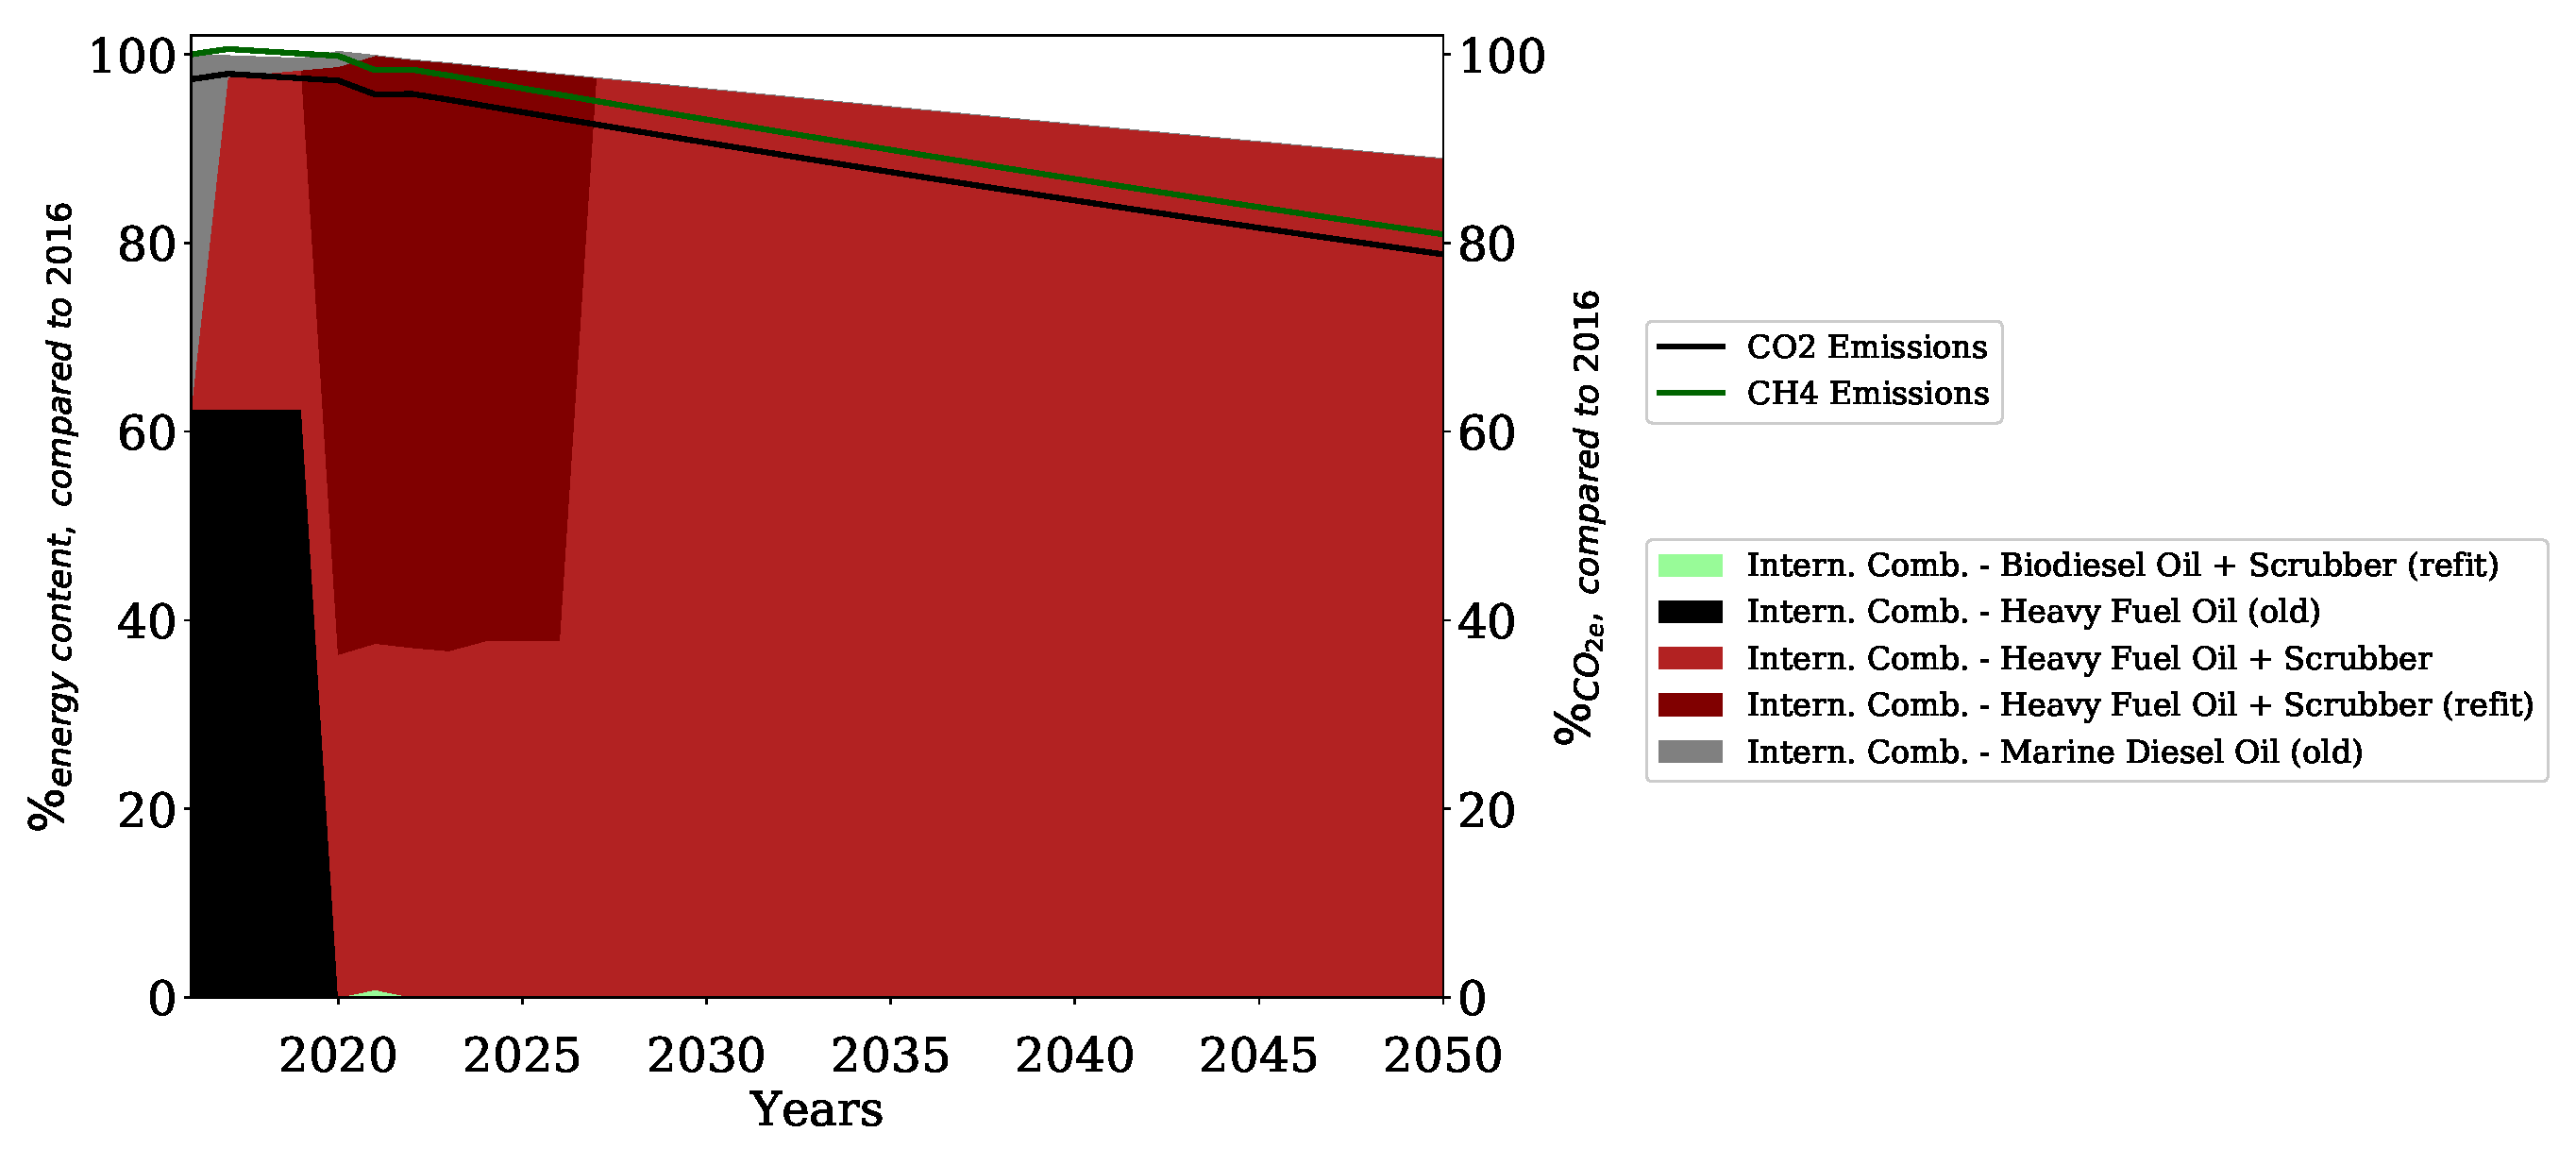
\includegraphics[width=\textwidth]{figures/BAU_fuels_emissions.eps}
    \caption{Fuel consumption (y-axis left) and cumulative emissions (y-axis right) in the business-as-usual scenario without carbon restrictions.}
    \label{fig:BAU}
\end{figure}
\begin{figure}[h]
    \centering
    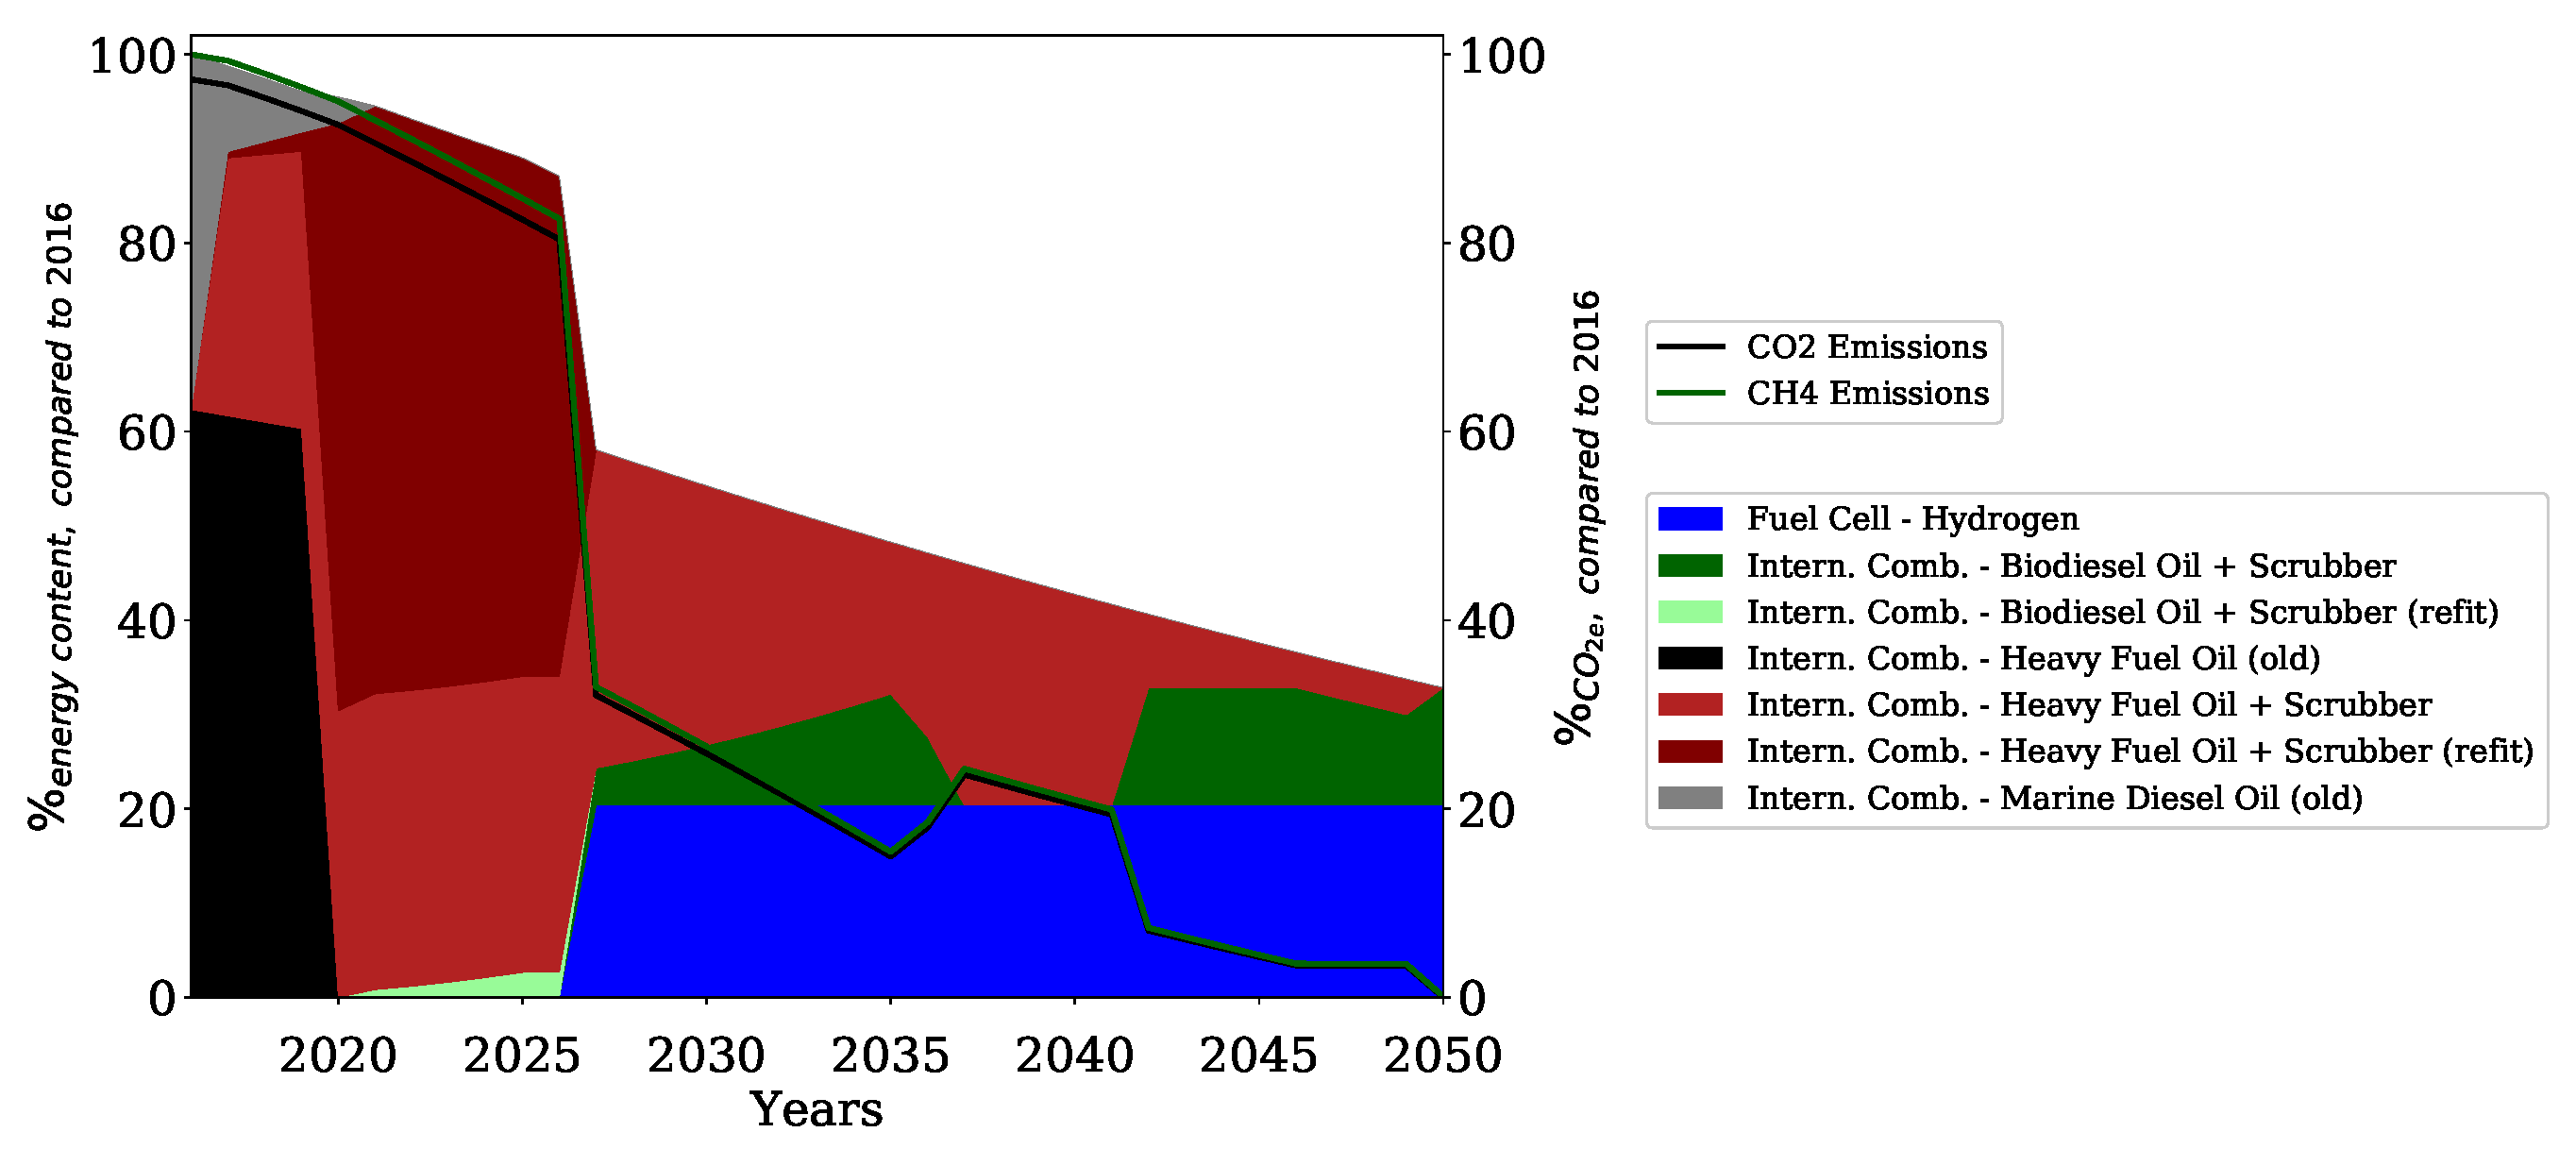
\includegraphics[width=\textwidth]{figures/TDVAR_fuels_emissions.eps}
    \caption{Fuel consumption (y-axis left) and cumulative emissions (y-axis right) in the reduced transport demand scenario with a limited carbon budget and assuming methane leakage phase-out.}
    \label{fig:TDV}
\end{figure}
\begin{figure}[h]
    \centering
    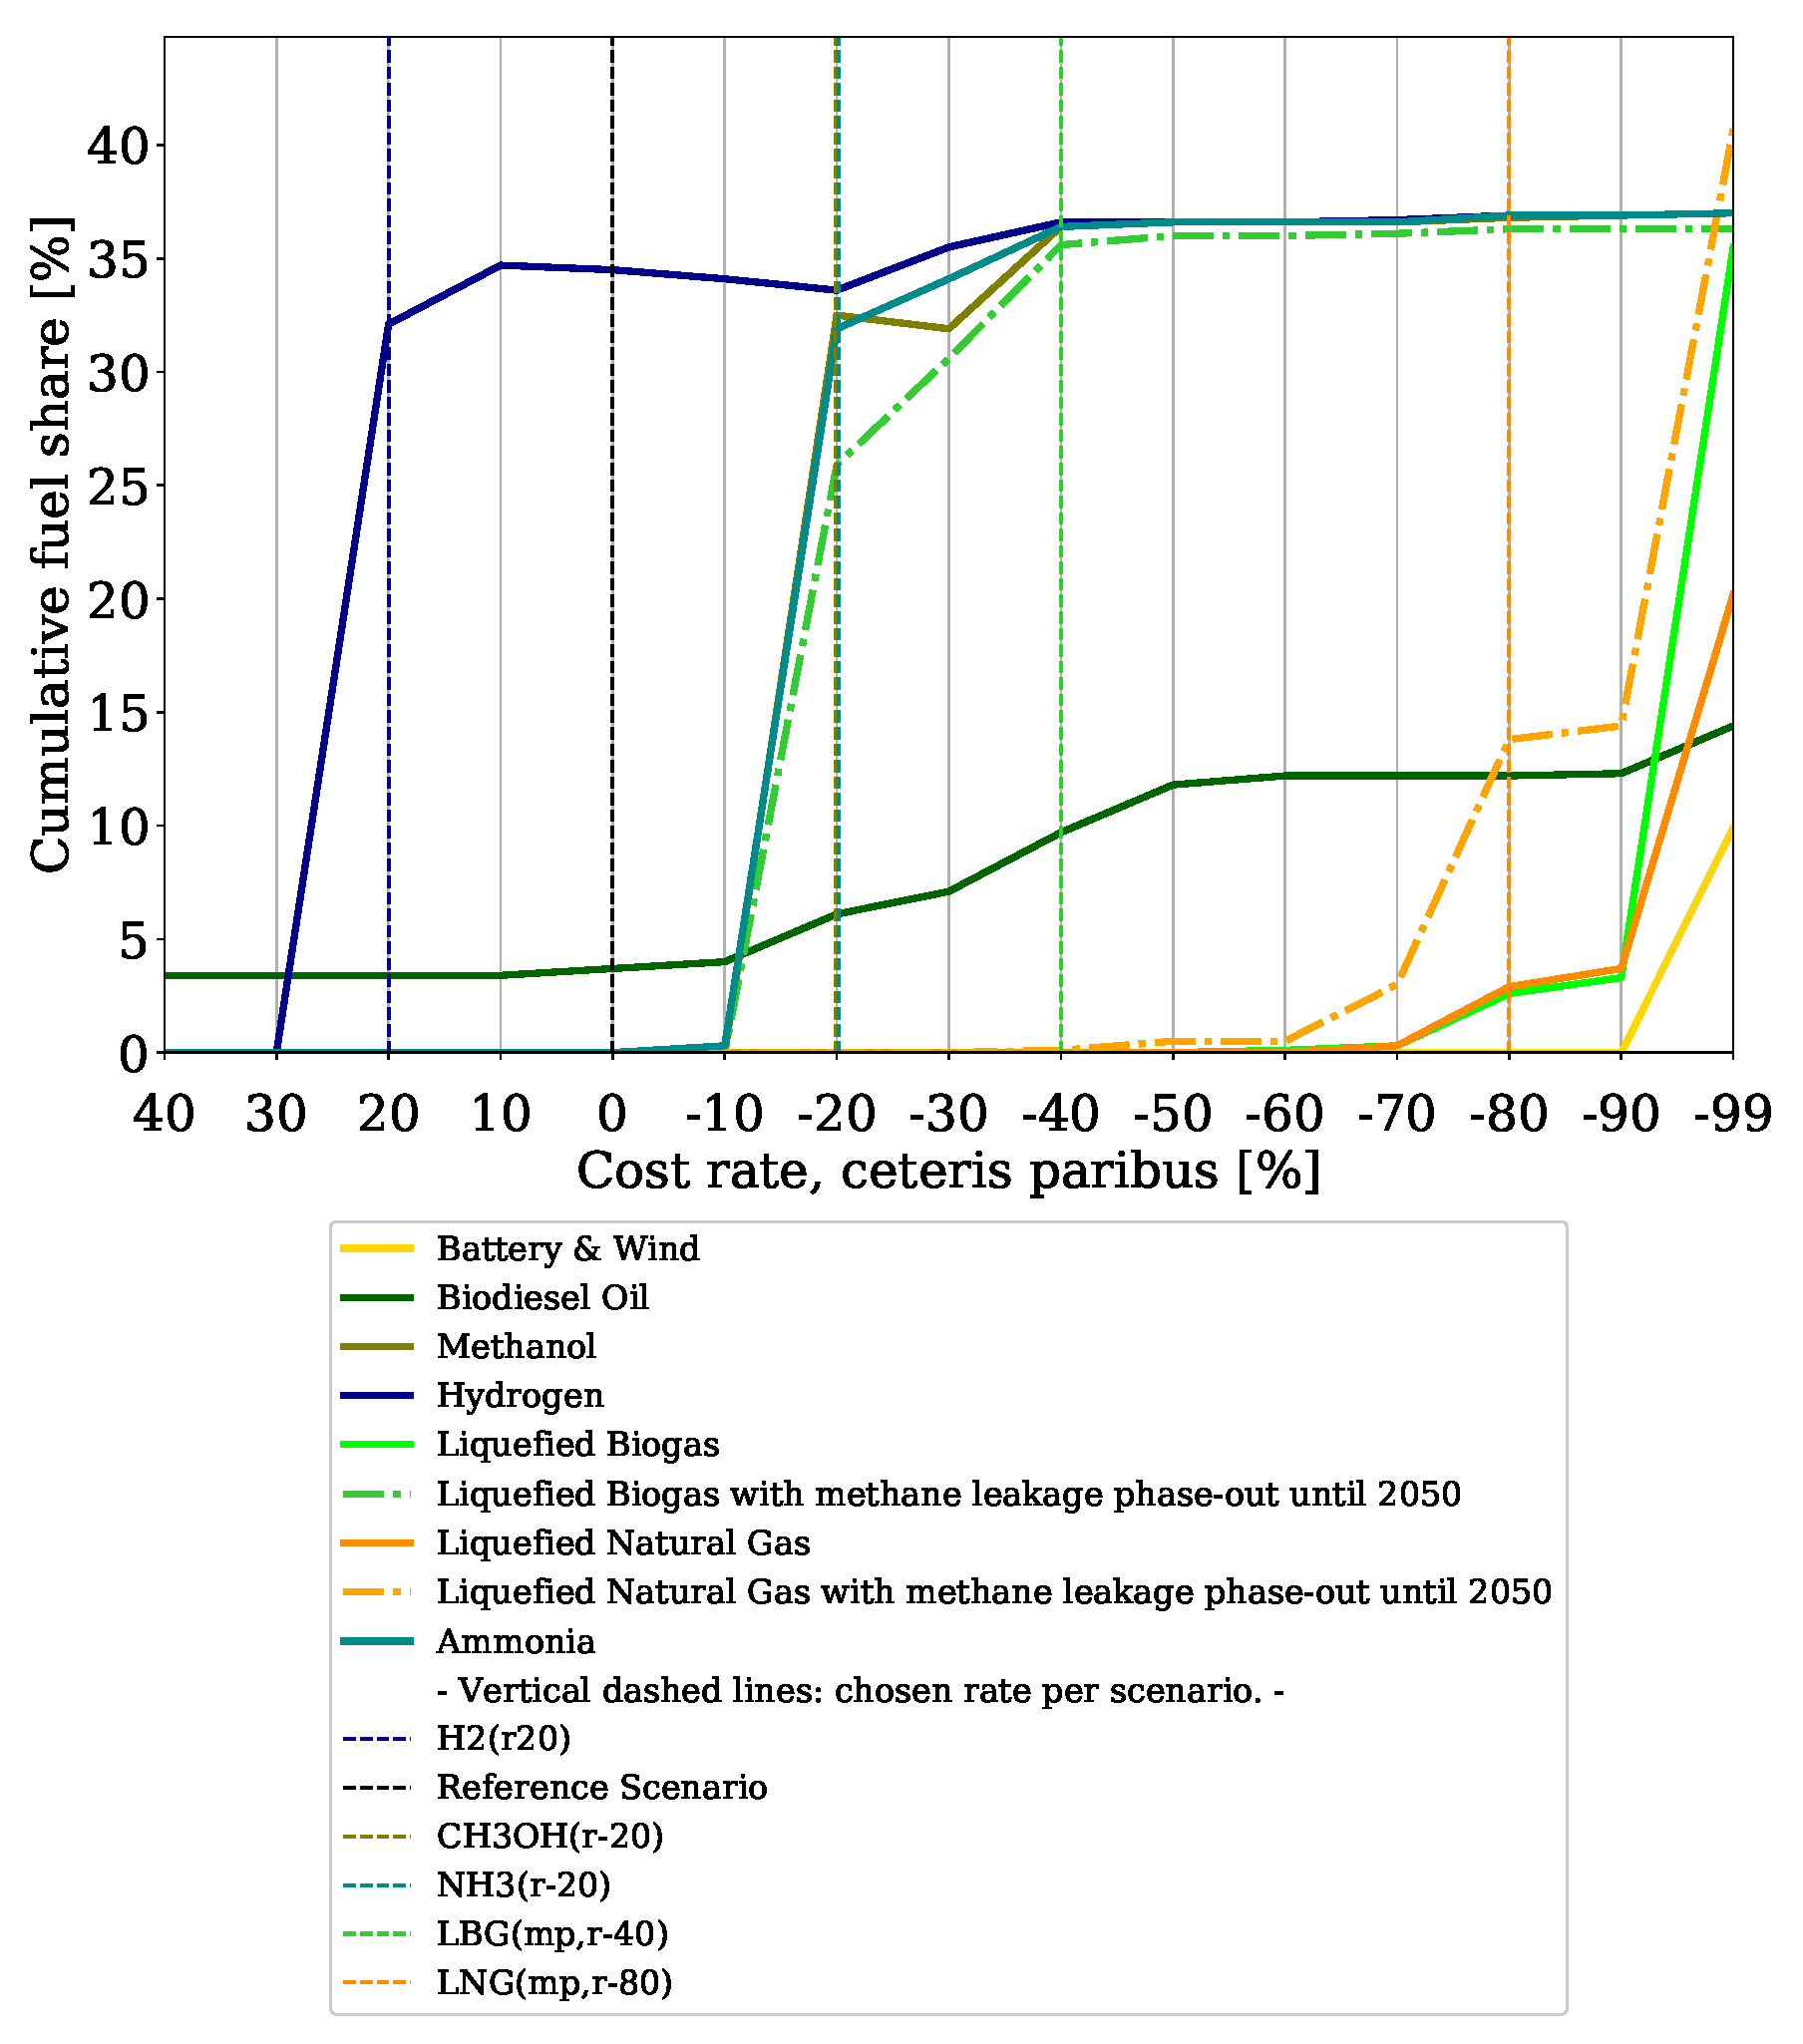
\includegraphics[width=.825\textwidth]{figures/costVariation.eps}
    \caption{Total fuel shares from 2016-2050 (y-axis) in relation to different cost range changes (x-axis) compared to the reference case.}
    \label{fig:costVariation}
\end{figure}
\begin{figure}[h]
    \centering
    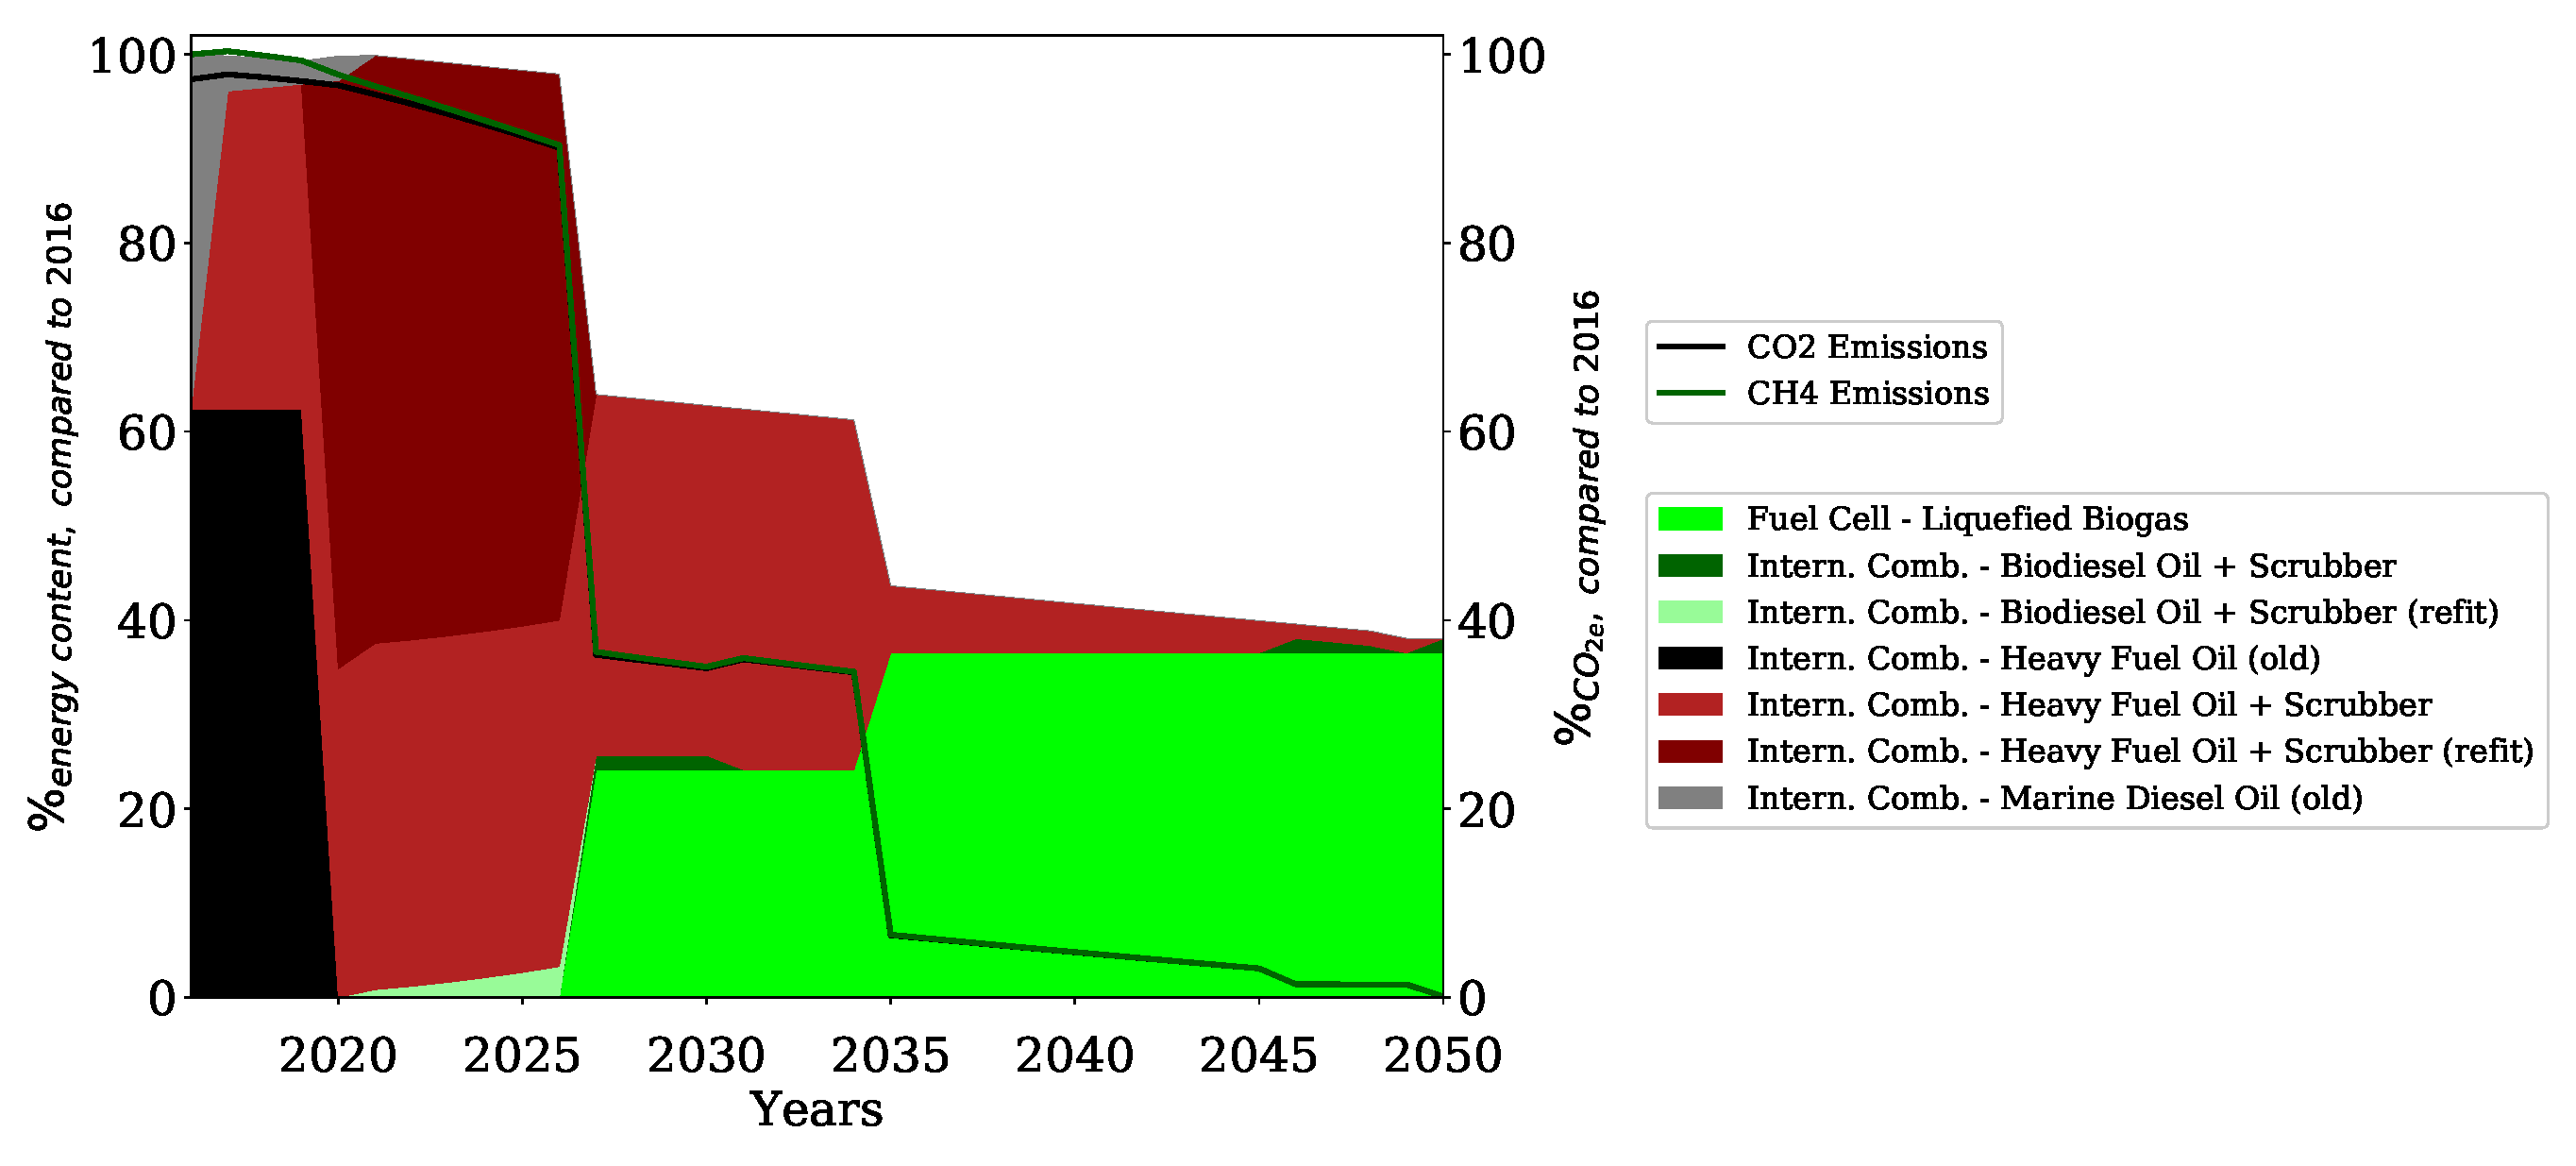
\includegraphics[width=\textwidth]{figures/LBG_MP_fuels_emissions.eps}
    \caption{Fuel consumption (y-axis left) and cumulative emissions (y-axis right) in the bio-methane scenario (LBG(mp), r-40) and assuming methane leakage phase-out.}
    \label{fig:LBG}
\end{figure}

\end{document}